\chapter{Additional graphs and spectra}

\newpage
\section{NICS of all sunflowers}

\begin{figure*}[h]
\centering
\begin{subfigure}{5.5cm}\centering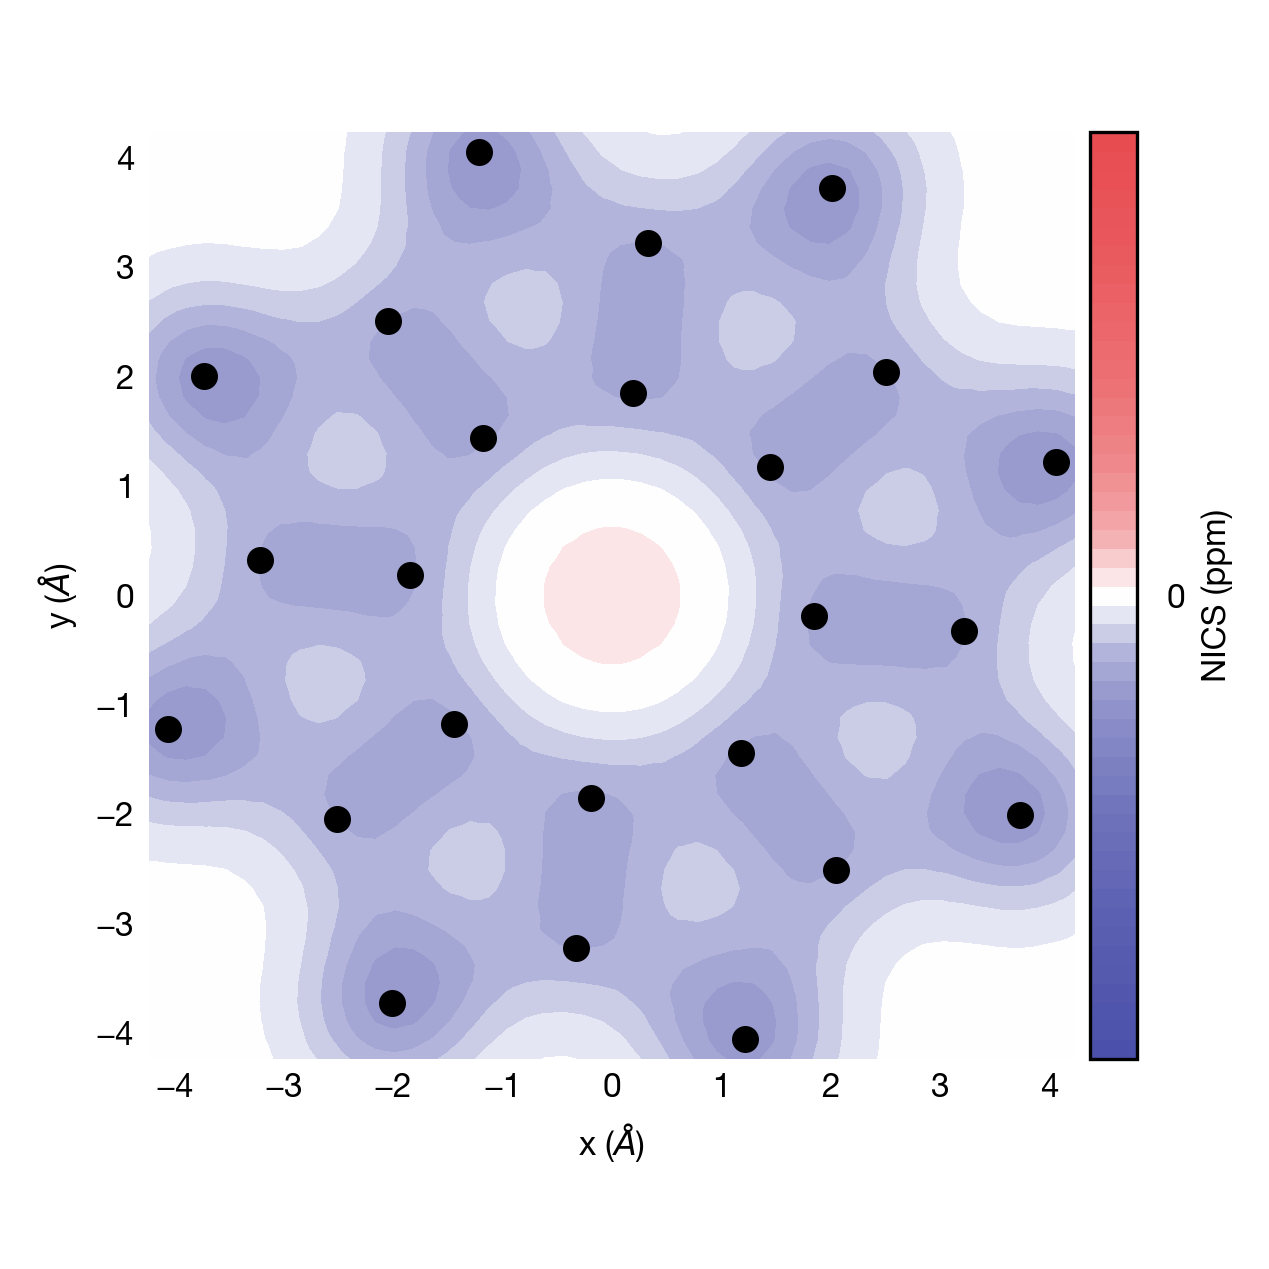
\includegraphics{s08-2d}\caption{NICS 2D projection for S08}\end{subfigure}%
\begin{subfigure}{5.5cm}\centering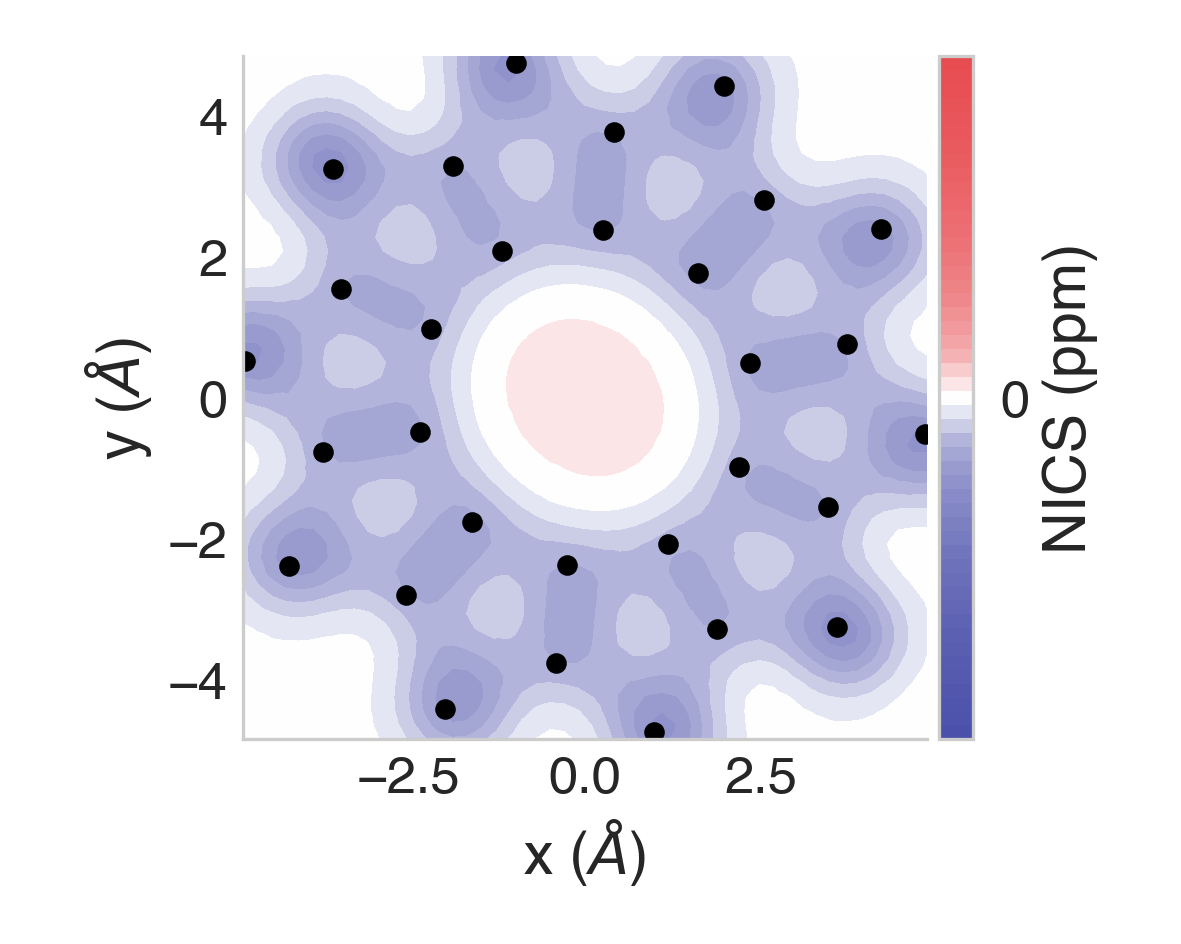
\includegraphics{s10-2d}\caption{NICS 2D projection for S10}\end{subfigure}%
\begin{subfigure}{5.5cm}\centering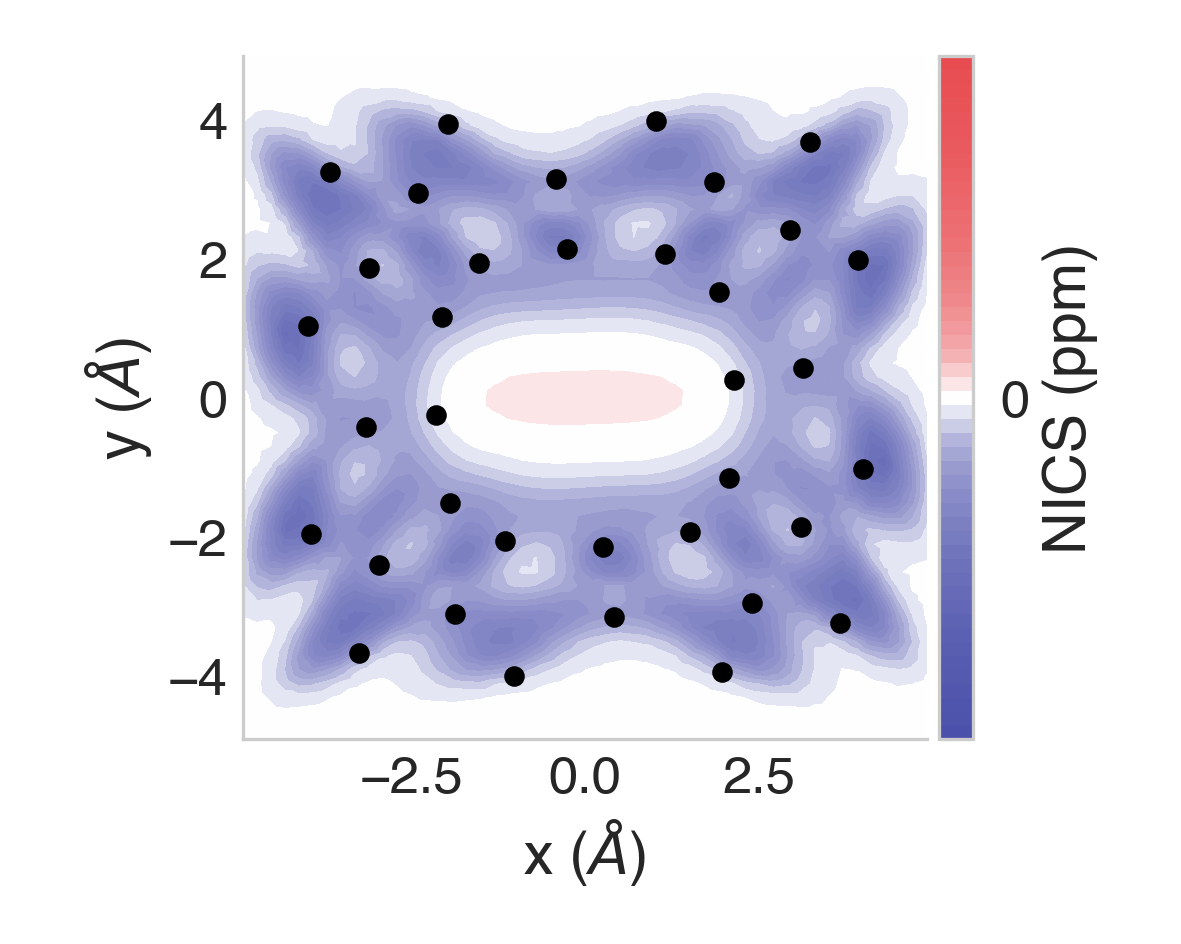
\includegraphics{s12-2d}\caption{NICS 2D projection for S12}\end{subfigure}
\begin{subfigure}{5.5cm}\centering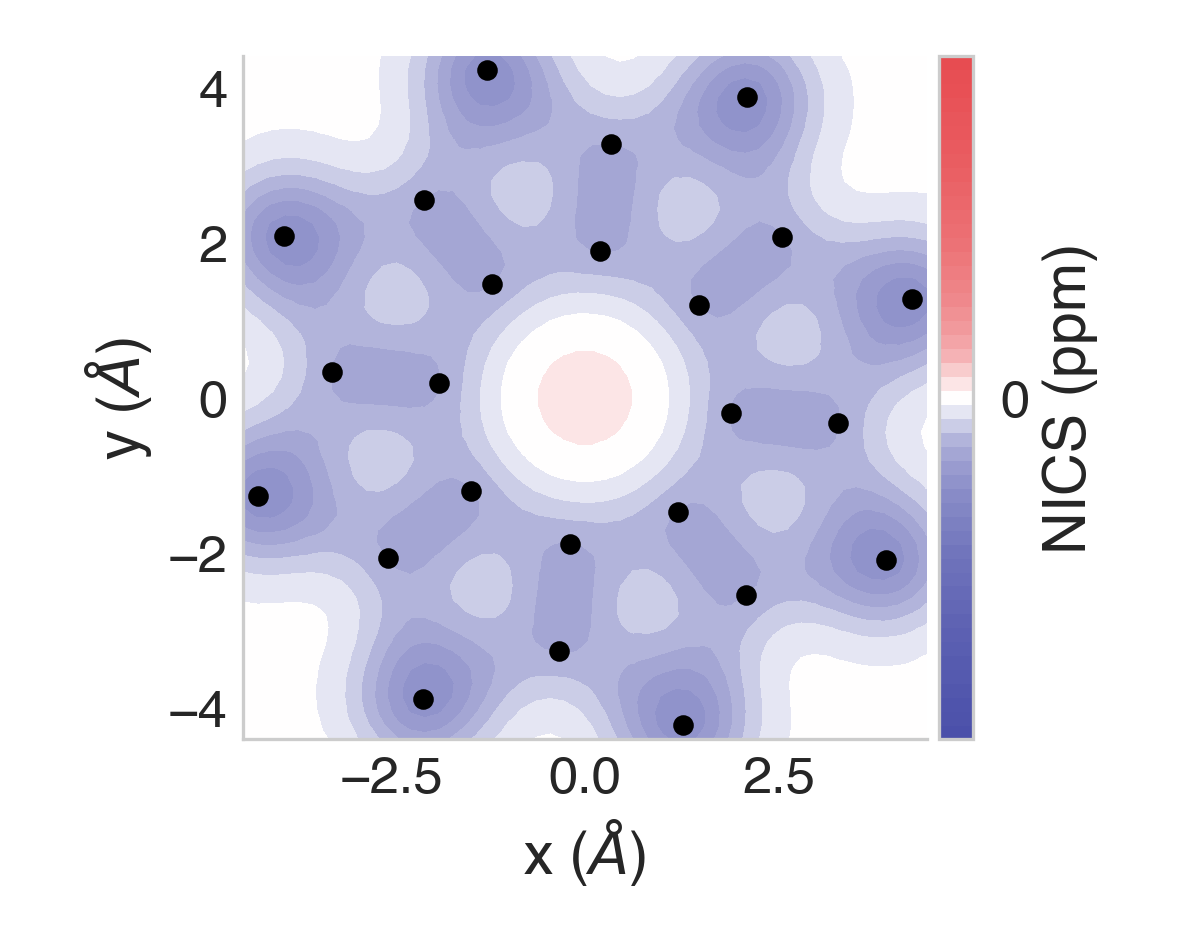
\includegraphics{se08-2d}\caption{NICS 2D projection for Se08}\end{subfigure}%
\begin{subfigure}{5.5cm}\centering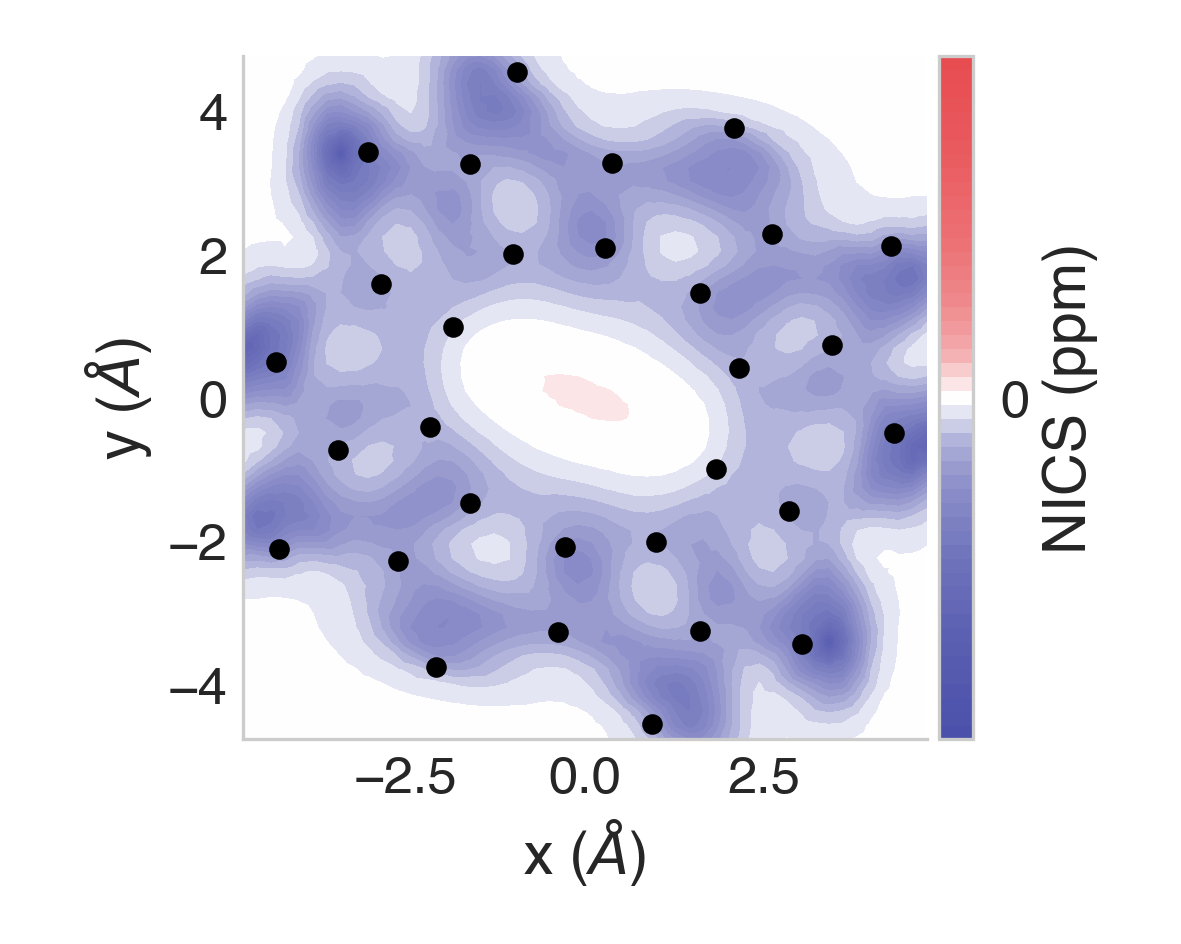
\includegraphics{se10-2d}\caption{NICS 2D projection for Se10}\end{subfigure}%
\begin{subfigure}{5.5cm}\centering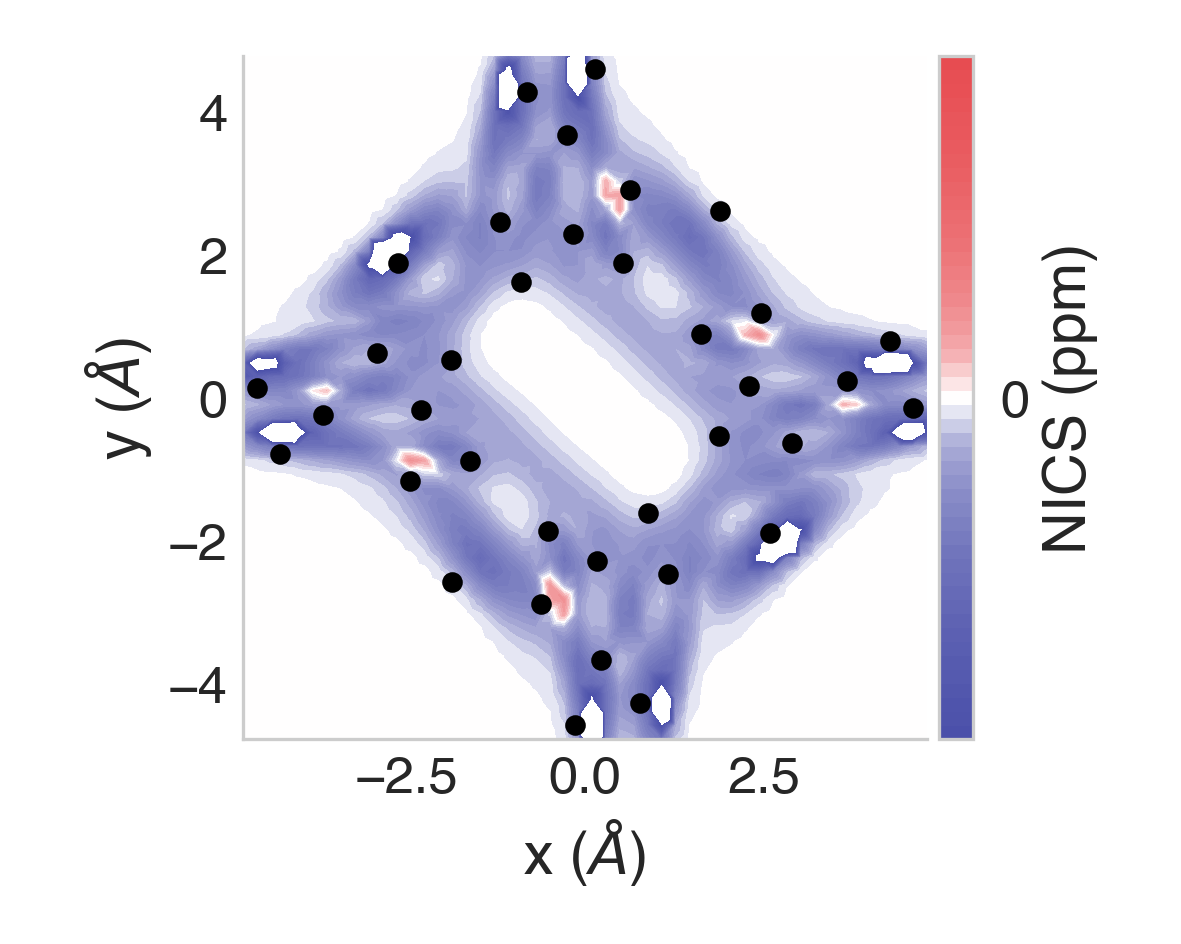
\includegraphics{se12-2d}\caption{NICS 2D projection for Se12}\end{subfigure}
\begin{subfigure}{5.5cm}\centering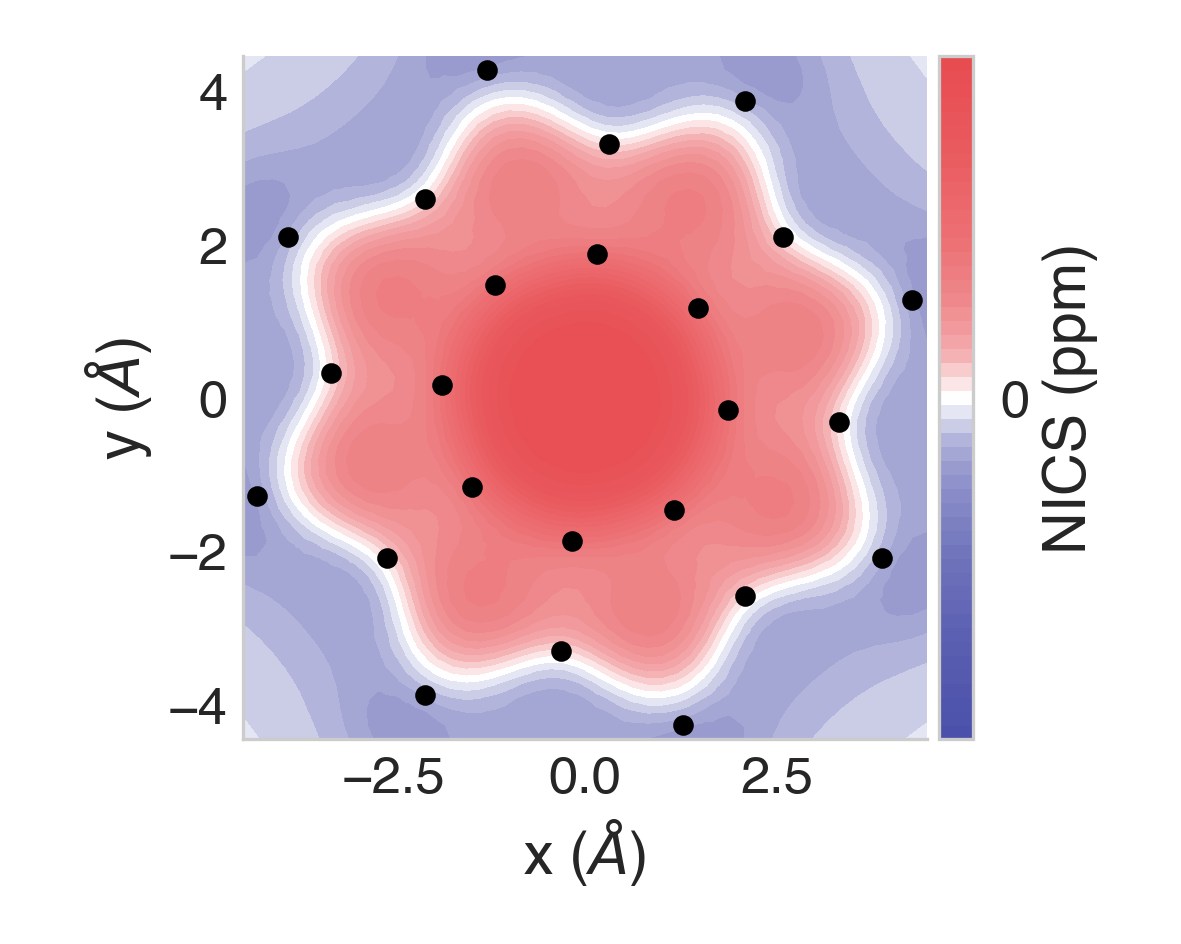
\includegraphics{as08-2d}\caption{NICS 2D projection for As08}\end{subfigure}%
\begin{subfigure}{5.5cm}\centering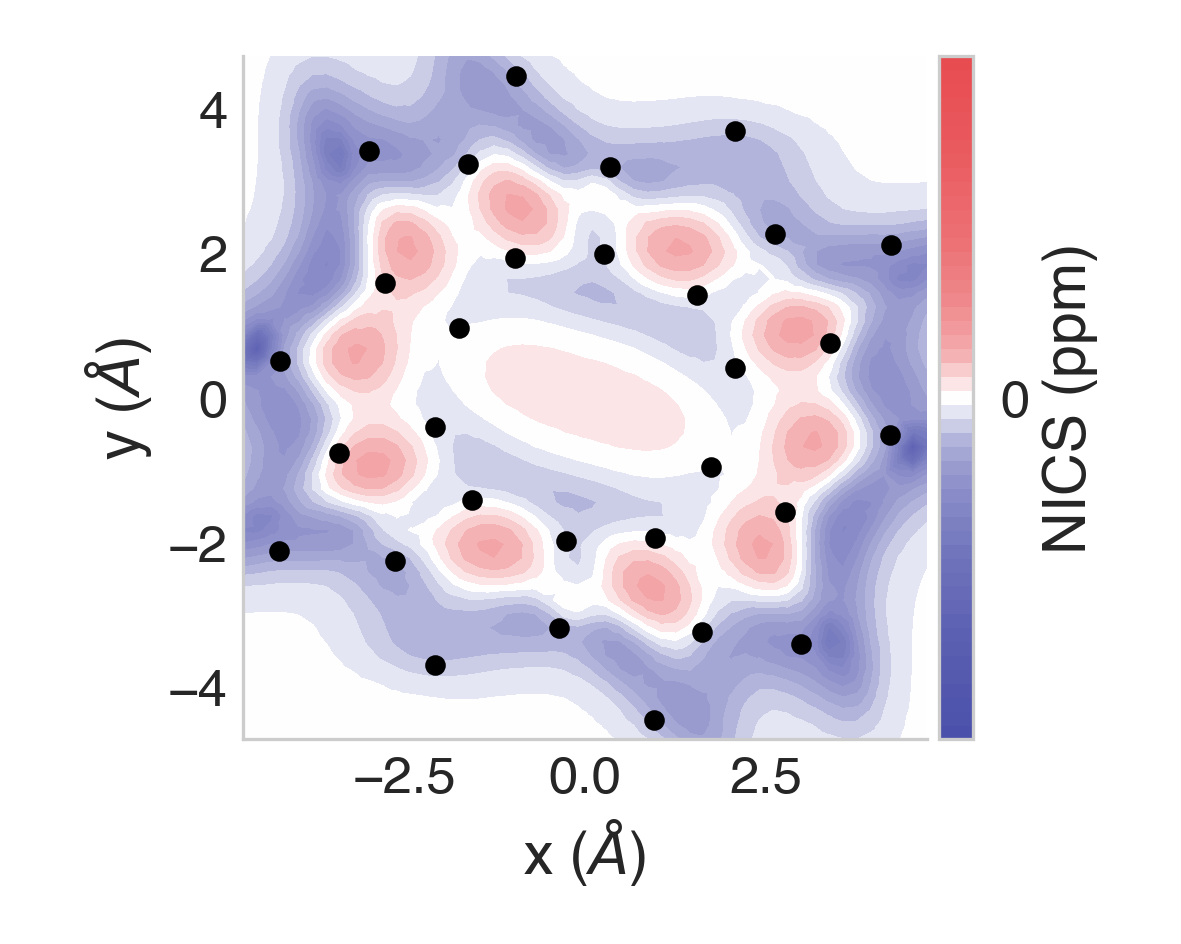
\includegraphics{as10-2d}\caption{NICS 2D projection for As10}\end{subfigure}%
\begin{subfigure}{5.5cm}\centering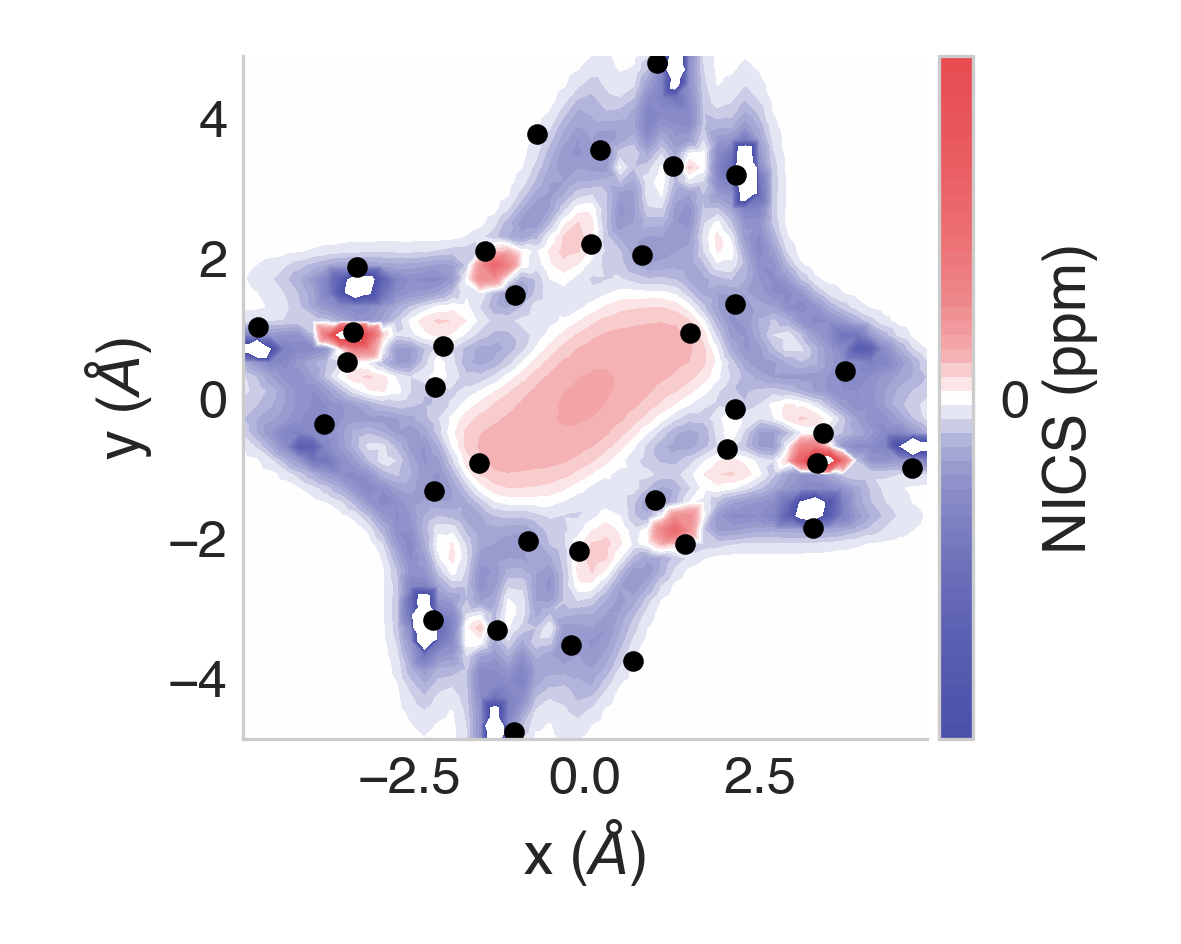
\includegraphics{as12-2d}\caption{NICS 2D projection for As12}\end{subfigure}
\caption[Part 1 of NICS 2D projections]{Part 1 of NICS 2D projections}
\end{figure*}

\newpage

\begin{figure*}[h]
\centering
\begin{subfigure}{5.5cm}\centering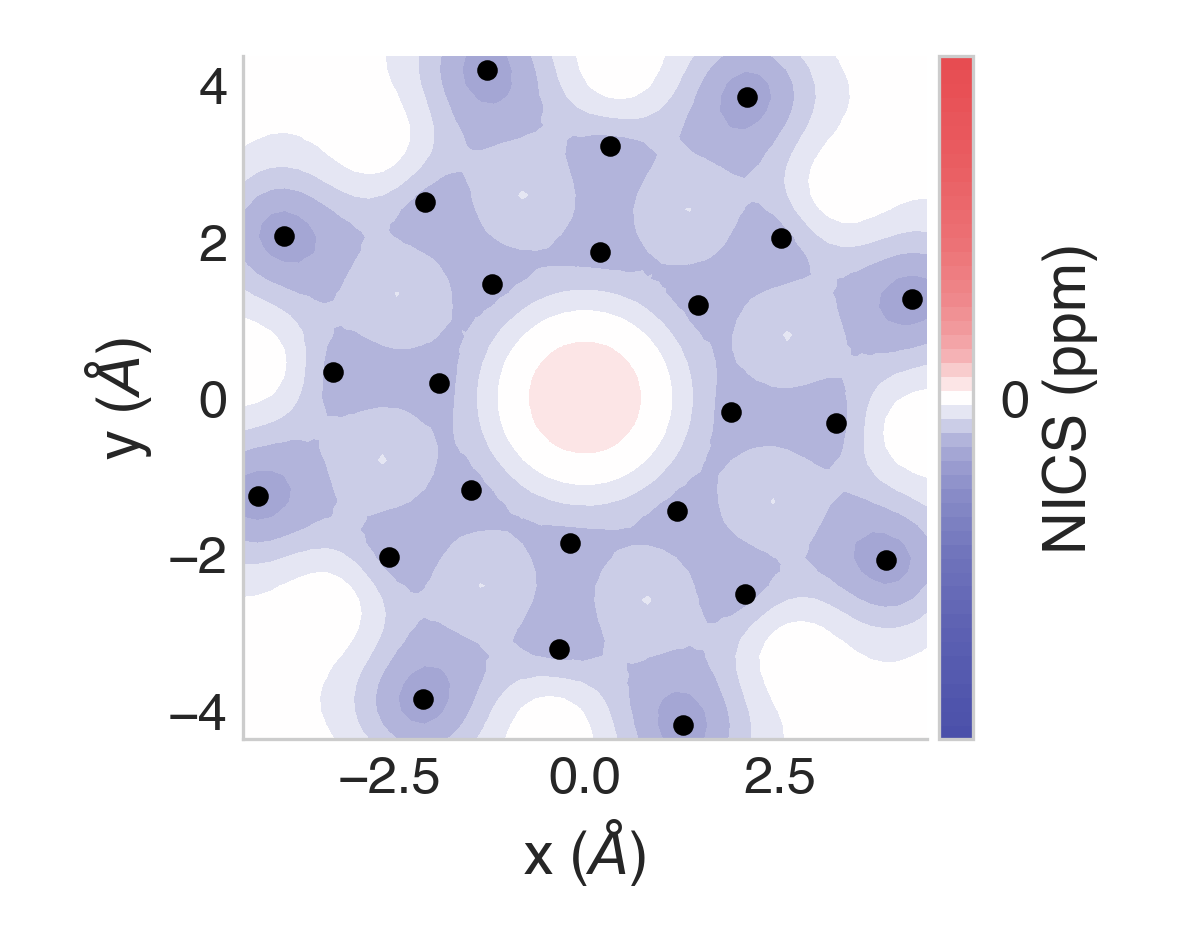
\includegraphics{asn08-2d}\caption{NICS 2D projection for AsN08}\end{subfigure}%
\begin{subfigure}{5.5cm}\centering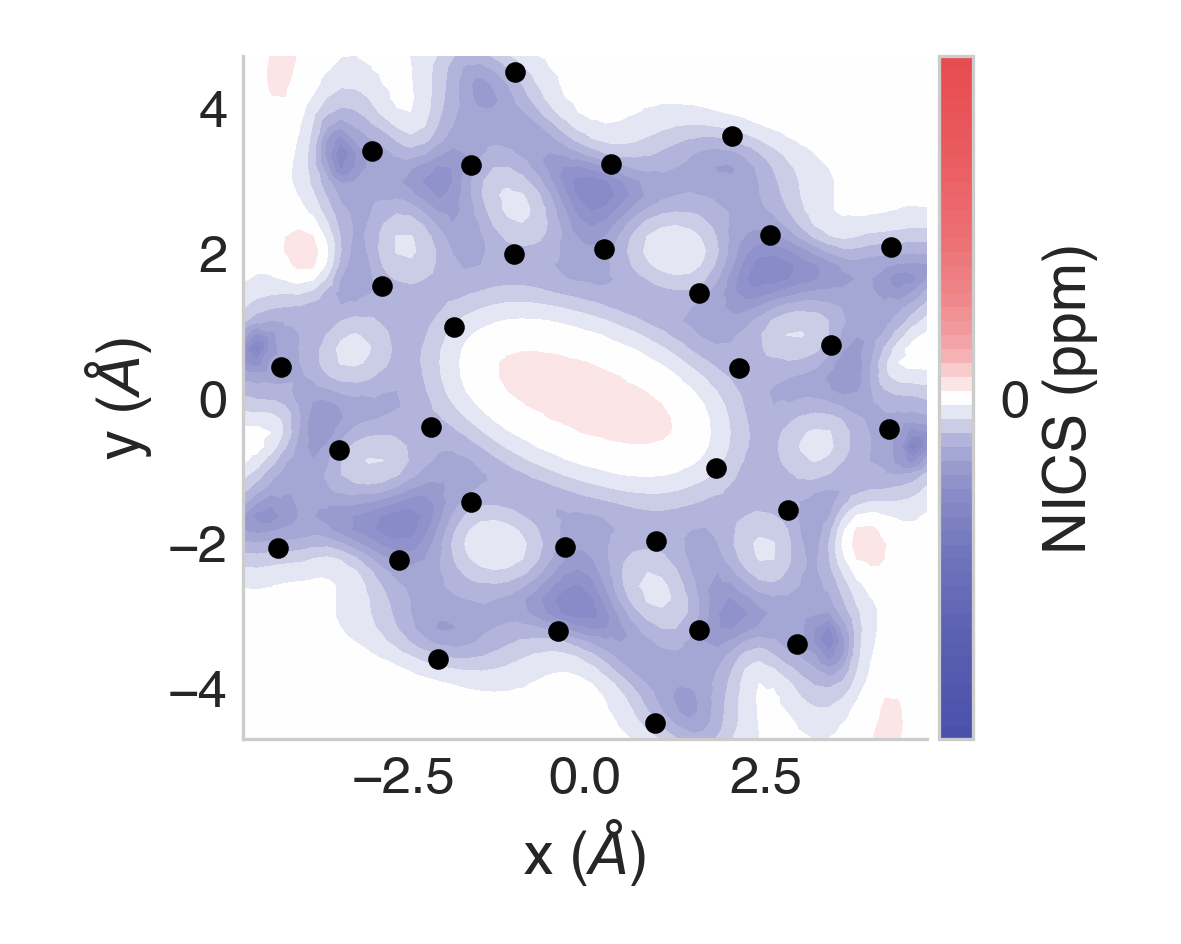
\includegraphics{asn10-2d}\caption{NICS 2D projection for AsN10}\end{subfigure}%
\begin{subfigure}{5.5cm}\centering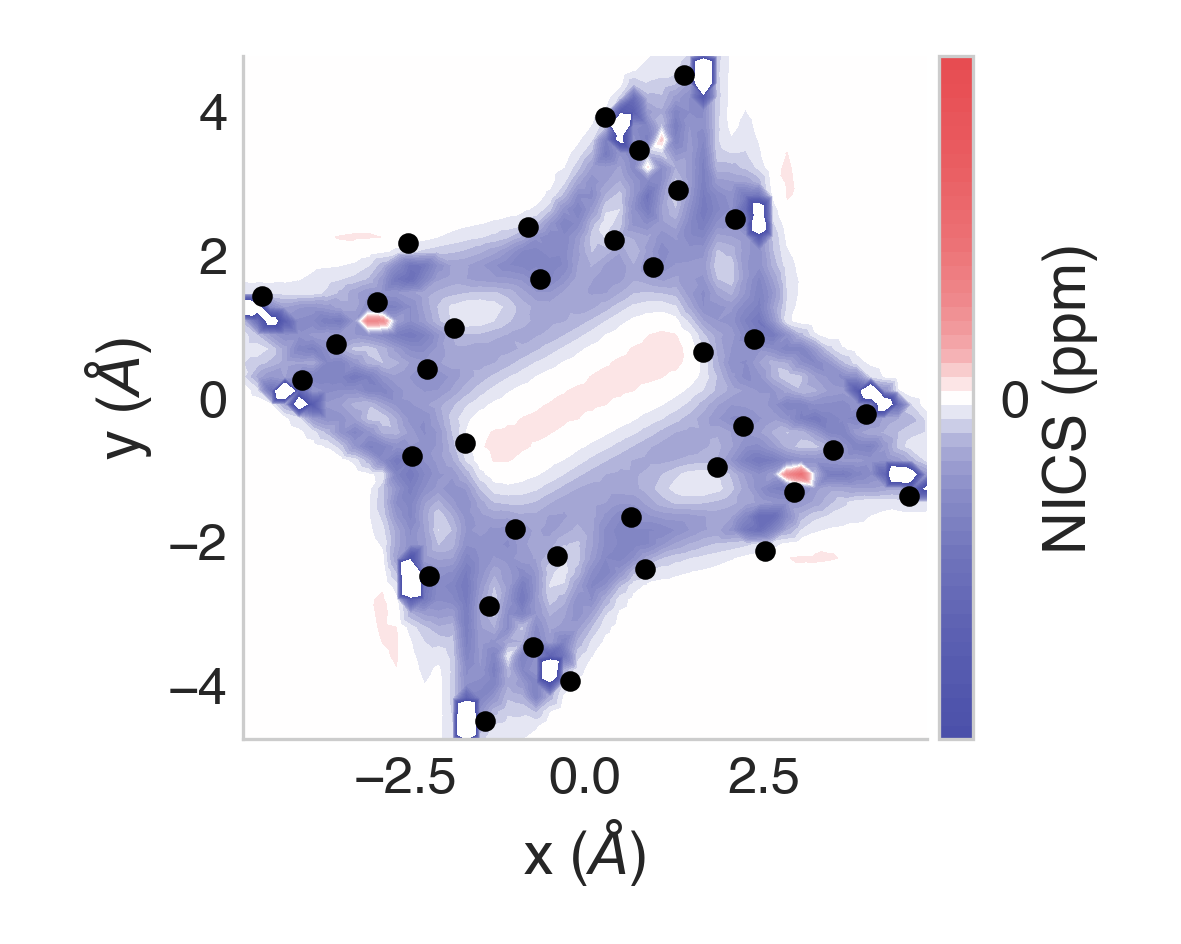
\includegraphics{asn12-2d}\caption{NICS 2D projection for AsN12}\end{subfigure}
\begin{subfigure}{5.5cm}\centering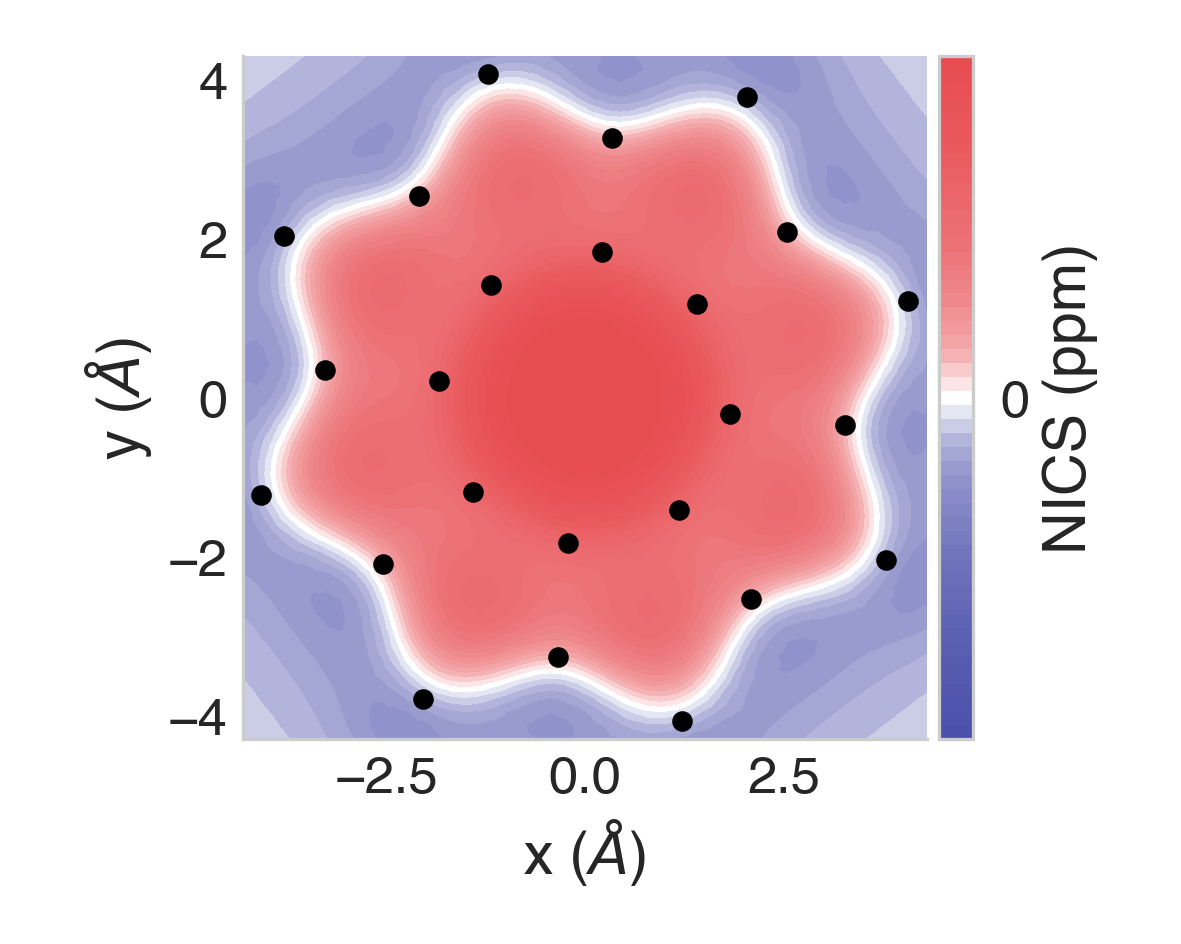
\includegraphics{p08-2d}\caption{NICS 2D projection for P08}\end{subfigure}%
\begin{subfigure}{5.5cm}\centering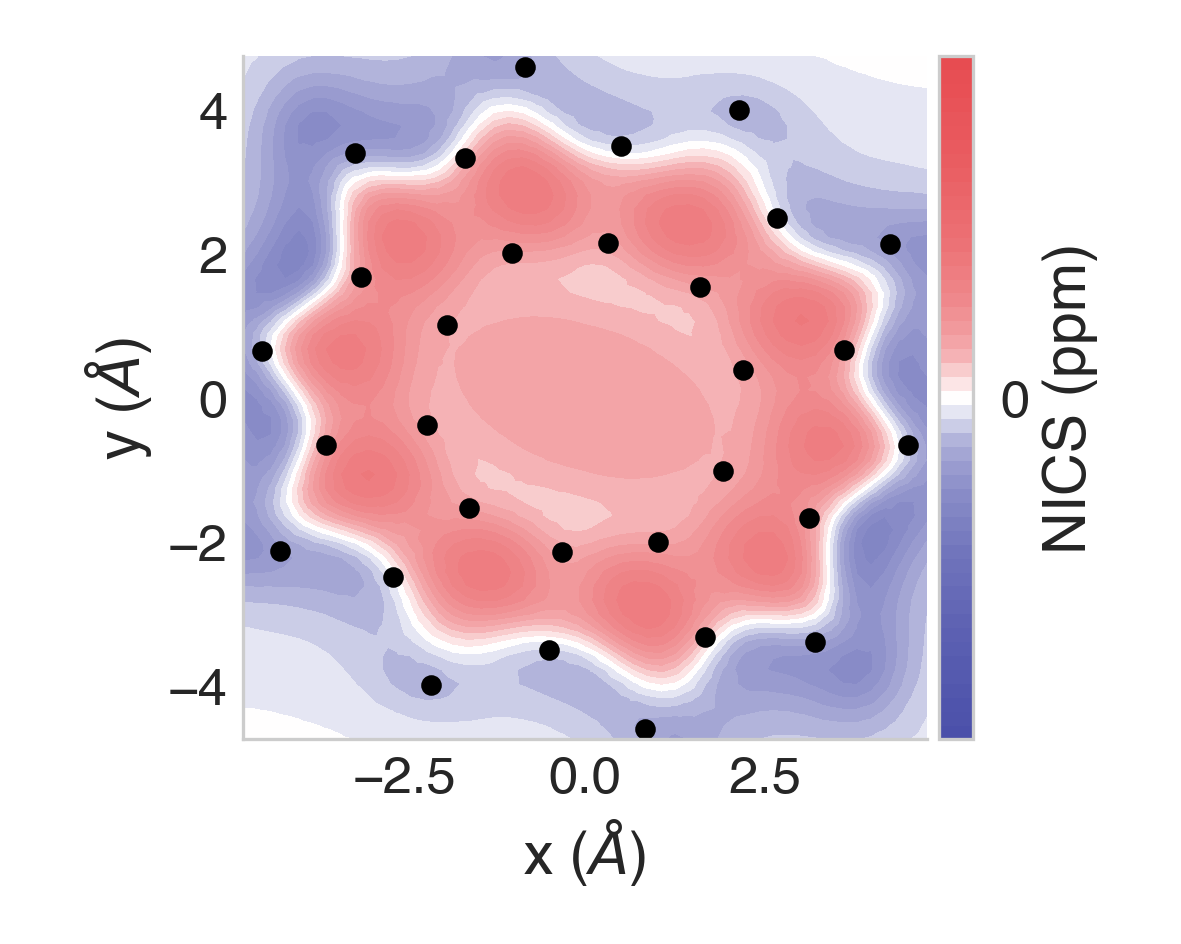
\includegraphics{p10-2d}\caption{NICS 2D projection for P10}\end{subfigure}%
\begin{subfigure}{5.5cm}\centering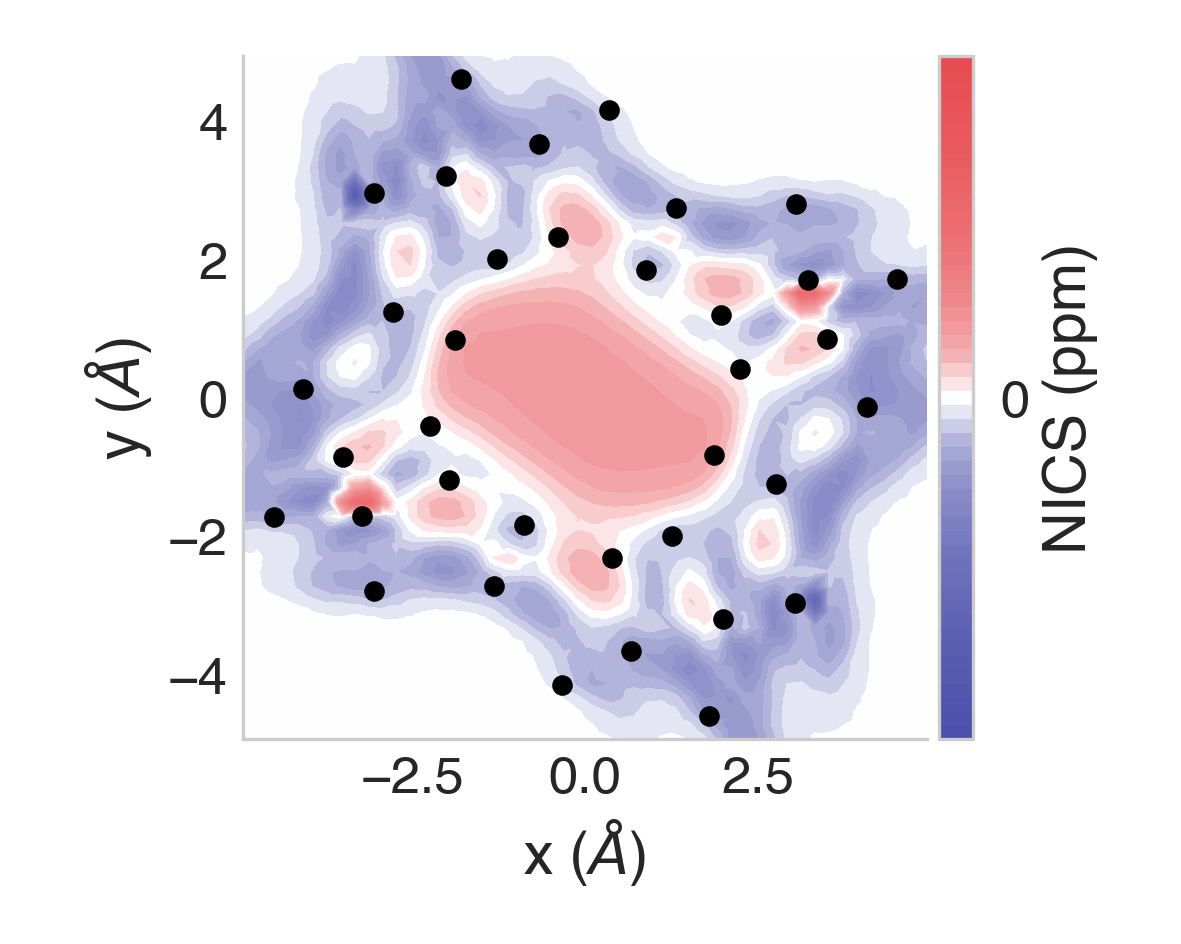
\includegraphics{p12-2d}\caption{NICS 2D projection for P12}\end{subfigure}
\begin{subfigure}{5.5cm}\centering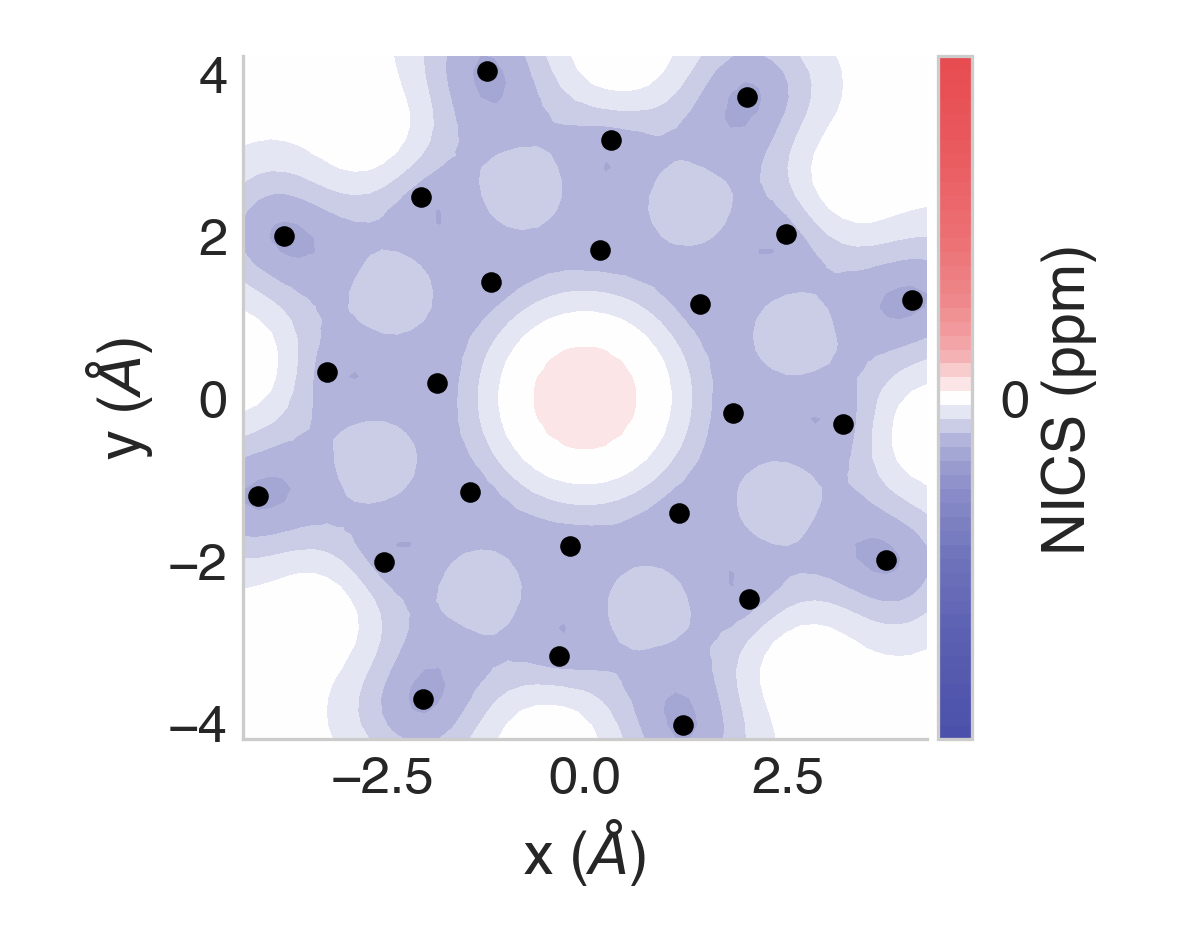
\includegraphics{pn08-2d}\caption{NICS 2D projection for PN08}\end{subfigure}%
\begin{subfigure}{5.5cm}\centering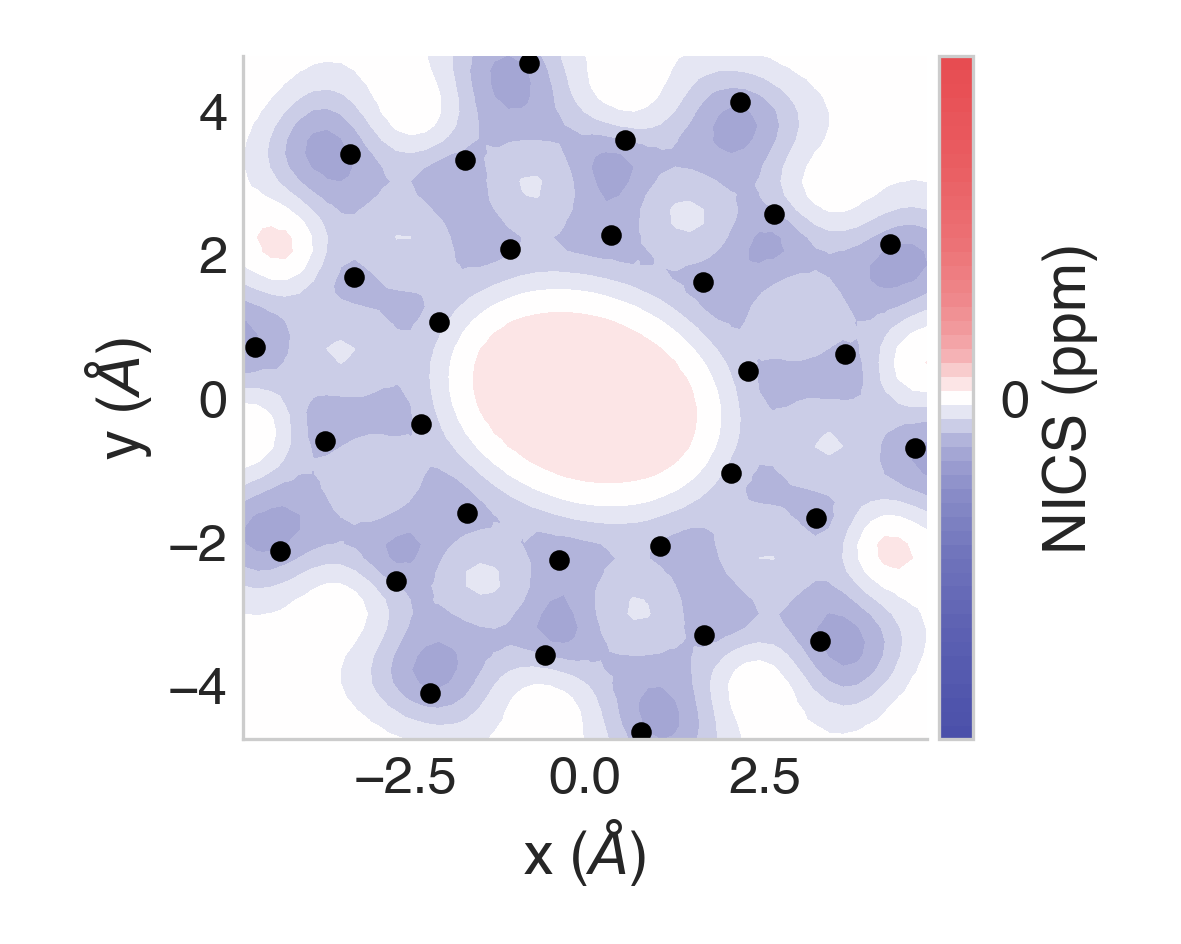
\includegraphics{pn10-2d}\caption{NICS 2D projection for PN10}\end{subfigure}%
\begin{subfigure}{5.5cm}\centering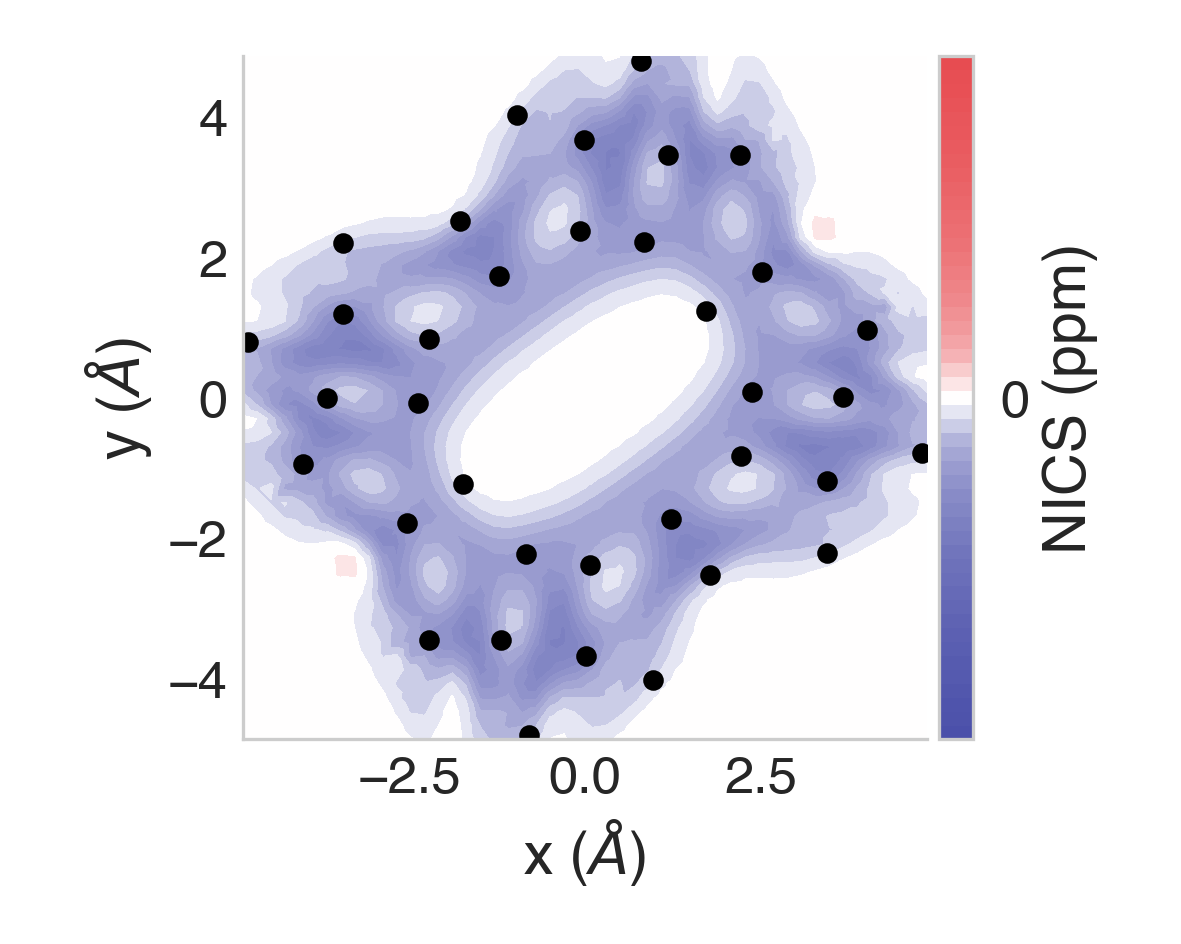
\includegraphics{pn12-2d}\caption{NICS 2D projection for PN12}\end{subfigure}
\caption[Part 2 of NICS 2D projections]{Part 2 of NICS 2D projections}
\end{figure*}


\newpage
\section{Raman spectra of all sunflowers}


\newpage
\section{UV-vis spectra of all sunflowers}
\labsec{ap:uv-vis-flowers}

\begin{figure*}[h]
\centering
\begin{subfigure}{8.25cm}\centering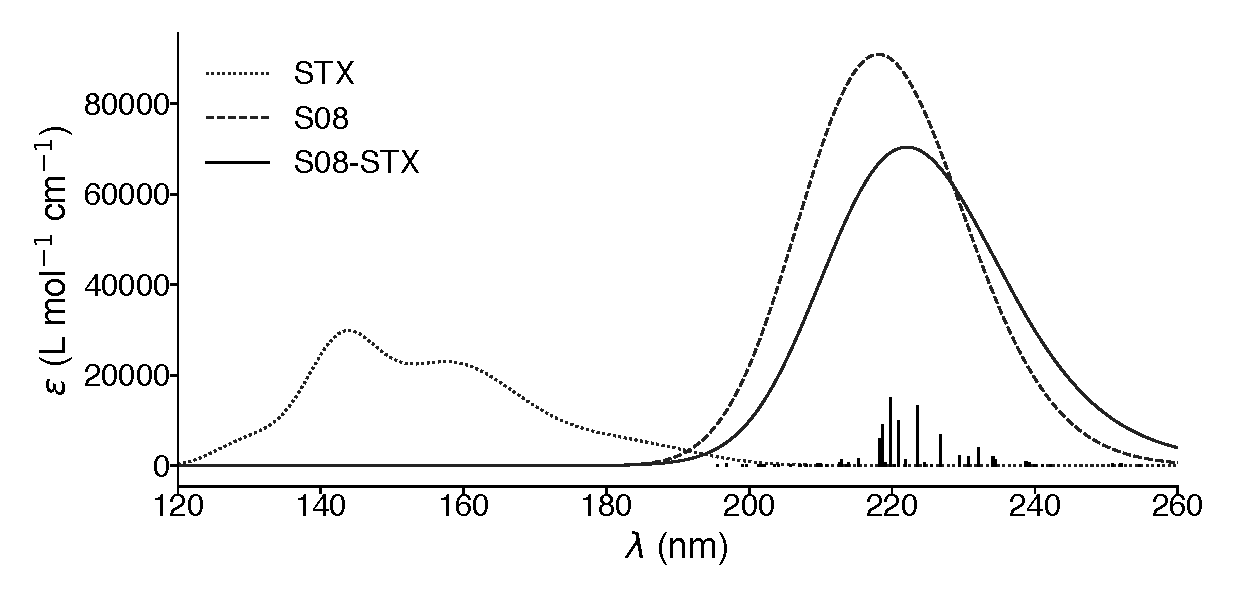
\includegraphics{uv-s08}\caption{UV-vis spectrum for S08}\end{subfigure}%
\begin{subfigure}{8.25cm}\centering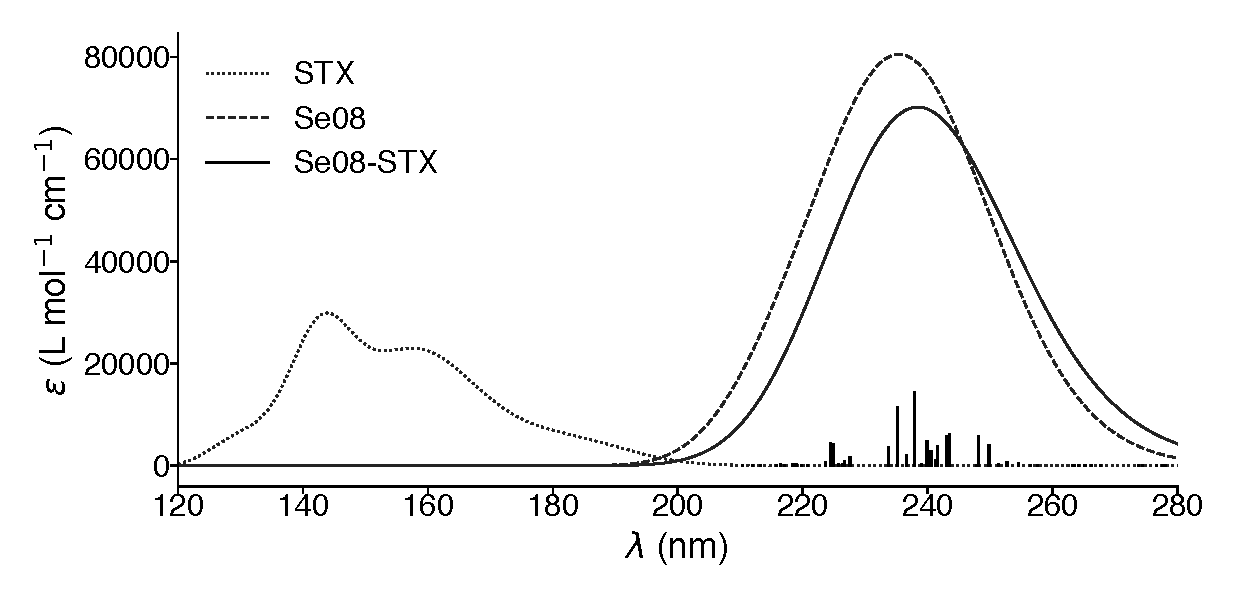
\includegraphics{uv-se08}\caption{UV-vis spectrum for Se08}\end{subfigure}
\begin{subfigure}{8.25cm}\centering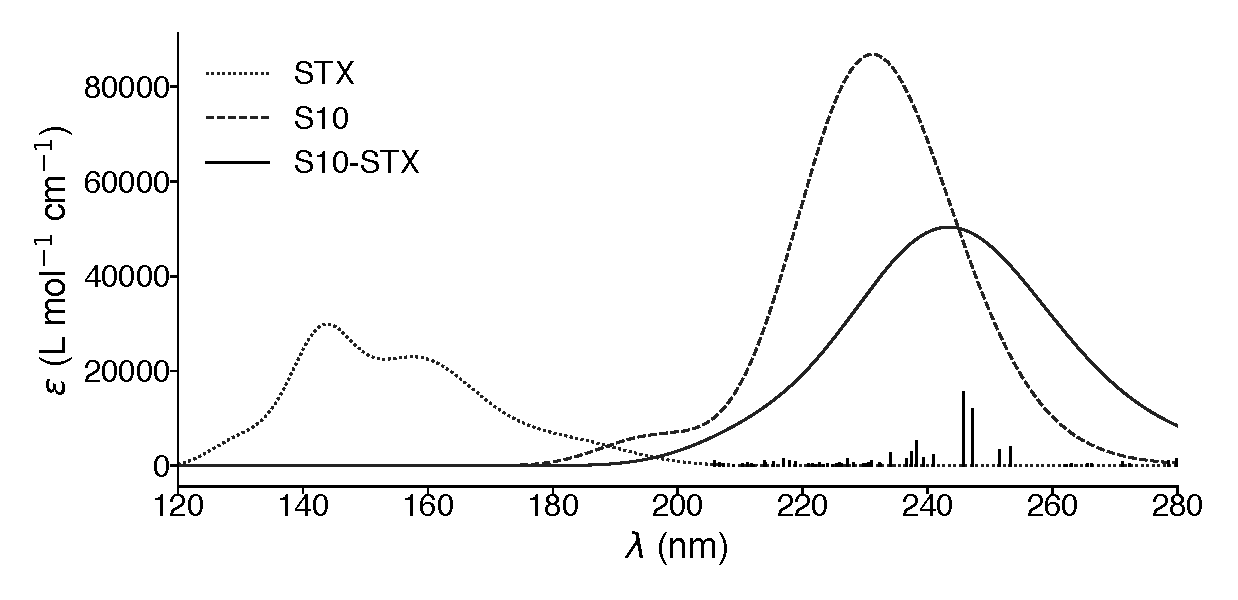
\includegraphics{uv-s10}\caption{UV-vis spectrum for S10}\end{subfigure}%
\begin{subfigure}{8.25cm}\centering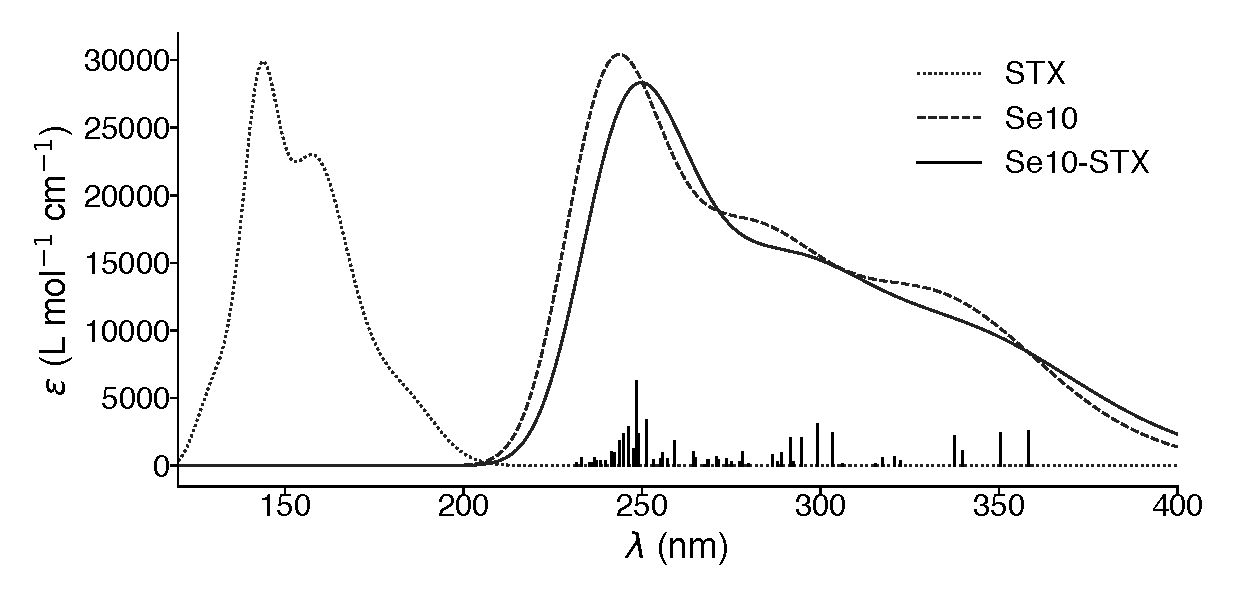
\includegraphics{uv-se10}\caption{UV-vis spectrum for Se10}\end{subfigure}
\begin{subfigure}{8.25cm}\centering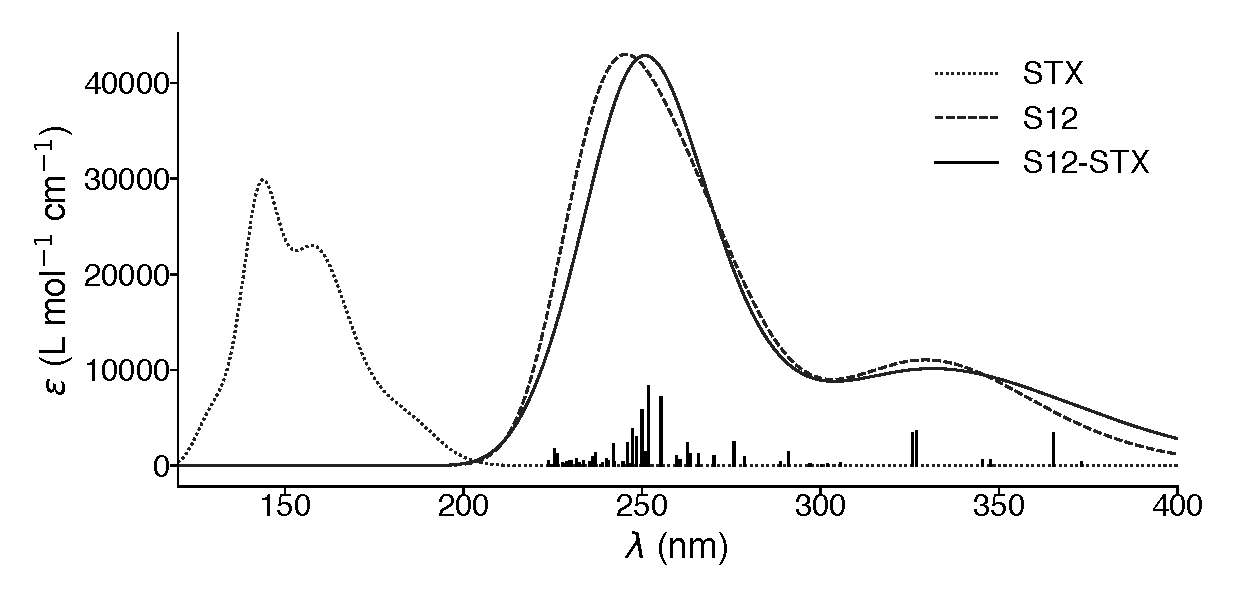
\includegraphics{uv-s12}\caption{UV-vis spectrum for S12}\end{subfigure}%
\begin{subfigure}{8.25cm}\centering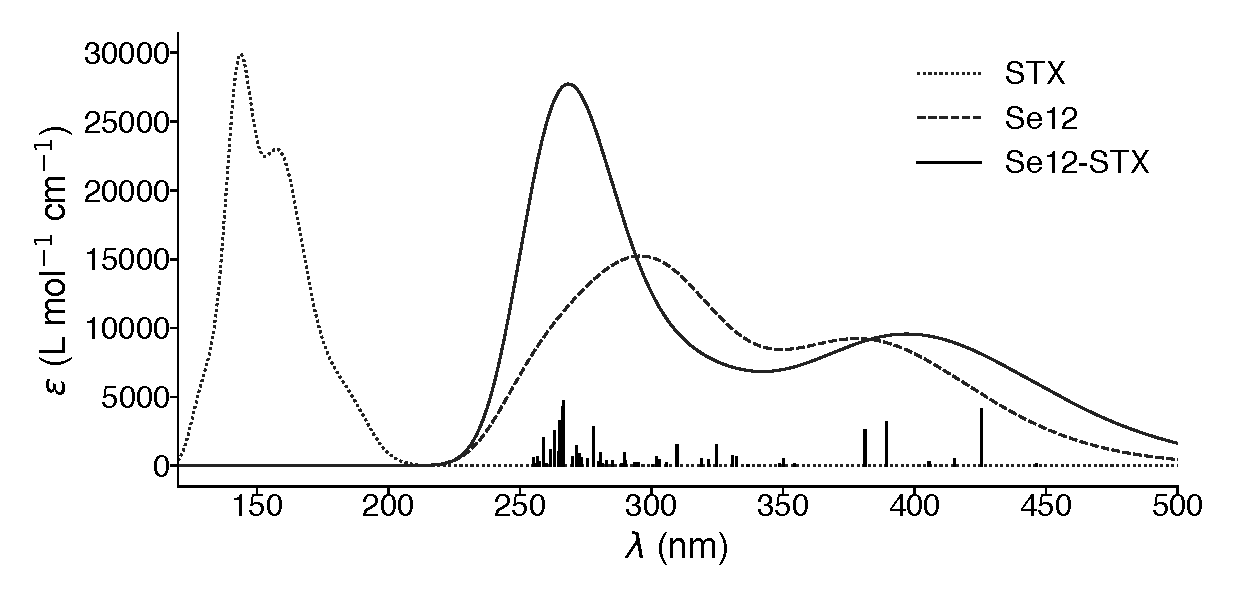
\includegraphics{uv-se12}\caption{UV-vis spectrum for Se12}\end{subfigure}
\caption[Part 1 of flower UV-vis spectra]{Part 1 of flower UV-vis spectra}
\end{figure*}

\newpage

\begin{figure*}[h]
\centering
\begin{subfigure}{8.25cm}\centering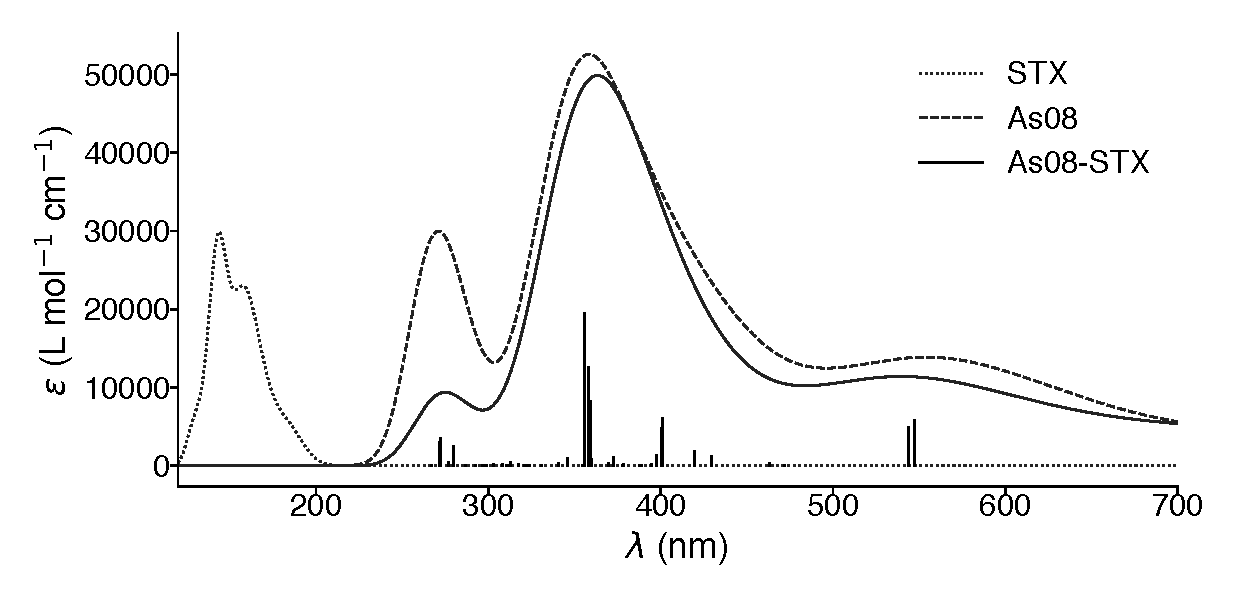
\includegraphics{uv-as08}\caption{UV-vis spectrum for As08}\end{subfigure}%
\begin{subfigure}{8.25cm}\centering\includegraphics{uv-asn08}\caption{UV-vis spectrum for AsN08}\end{subfigure}
\begin{subfigure}{8.25cm}\centering\includegraphics{uv-as10}\caption{UV-vis spectrum for As10}\end{subfigure}%
\begin{subfigure}{8.25cm}\centering\includegraphics{uv-asn10}\caption{UV-vis spectrum for AsN10}\end{subfigure}
\begin{subfigure}{8.25cm}\centering\includegraphics{uv-as12}\caption{UV-vis spectrum for As12}\end{subfigure}%
\begin{subfigure}{8.25cm}\centering\includegraphics{uv-asn12}\caption{UV-vis spectrum for AsN12}\end{subfigure}
\caption[Part 2 of flower UV-vis spectra]{Part 2 of flower UV-vis spectra}
\end{figure*}

\newpage

\begin{figure*}[h]
\centering
\begin{subfigure}{8.25cm}\centering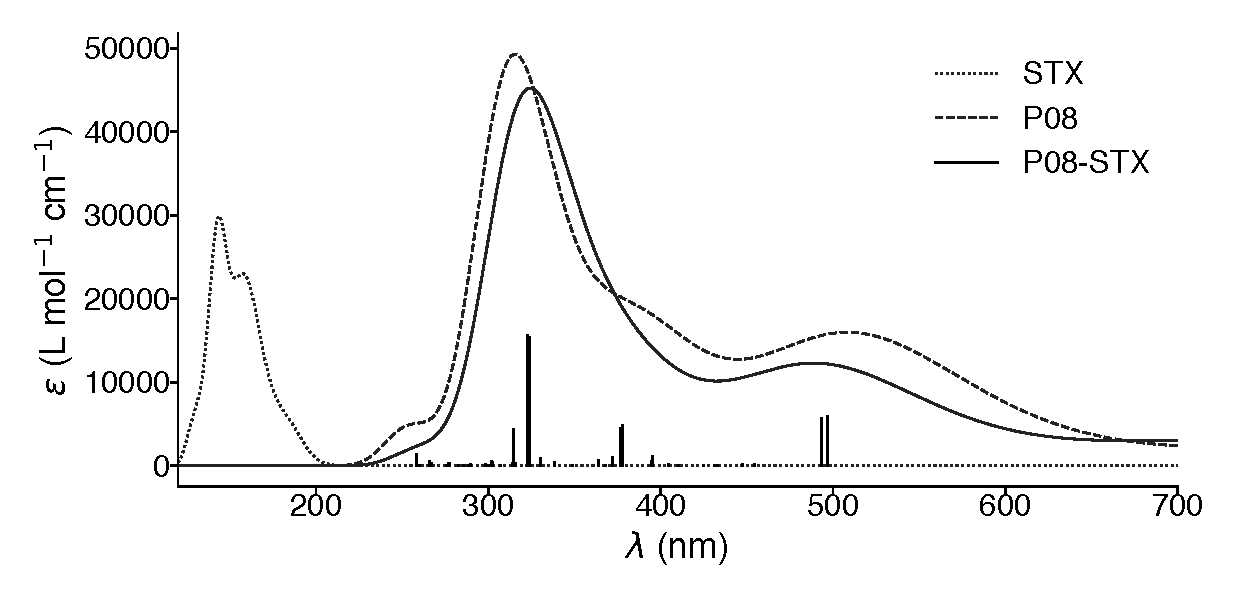
\includegraphics{uv-p08}\caption{UV-vis spectrum for P08}\end{subfigure}%
\begin{subfigure}{8.25cm}\centering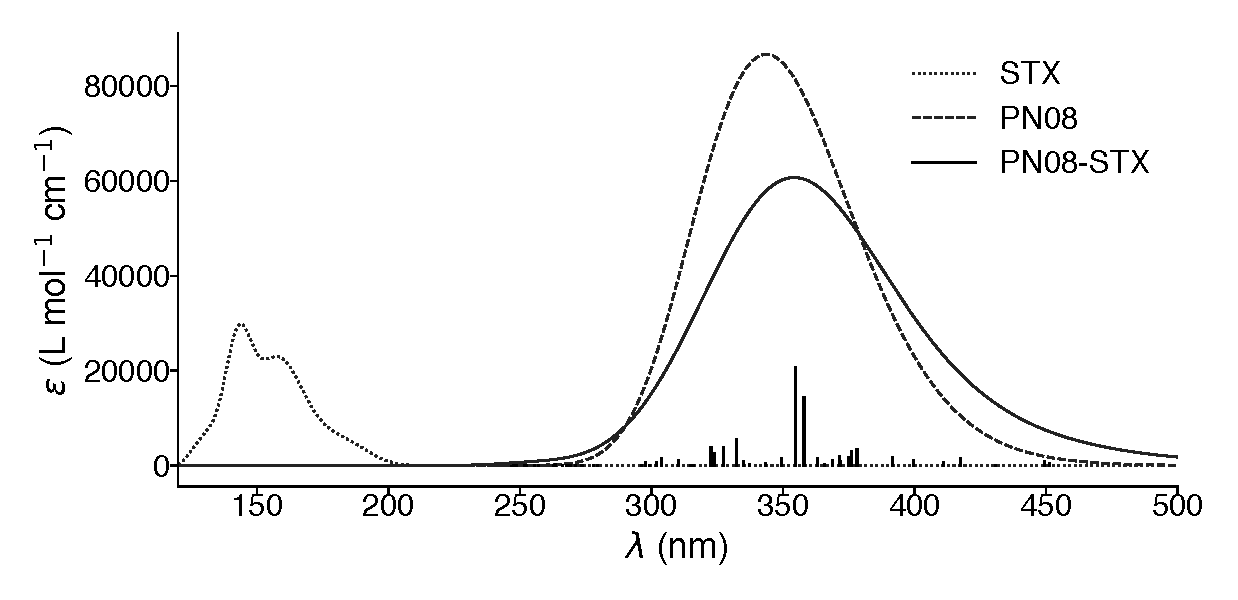
\includegraphics{uv-pn08}\caption{UV-vis spectrum for PN08}\end{subfigure}
\begin{subfigure}{8.25cm}\centering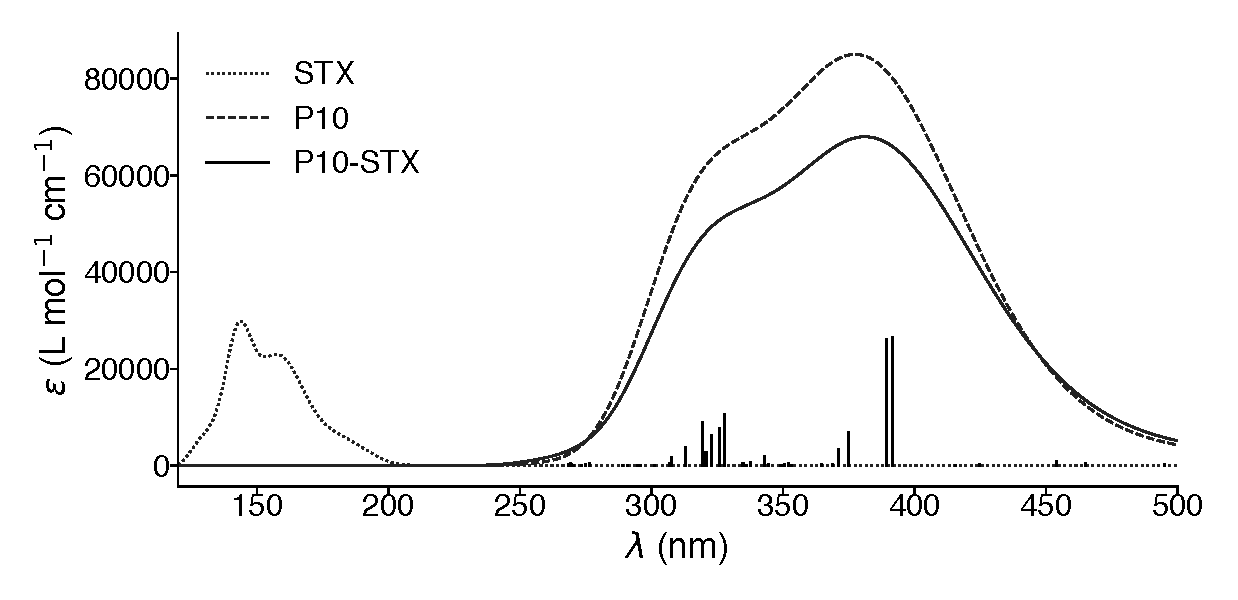
\includegraphics{uv-p10}\caption{UV-vis spectrum for P10}\end{subfigure}%
\begin{subfigure}{8.25cm}\centering\includegraphics{uv-pn10}\caption{UV-vis spectrum for PN10}\end{subfigure}
\begin{subfigure}{8.25cm}\centering\includegraphics{uv-p12}\caption{UV-vis spectrum for P12}\end{subfigure}%
\begin{subfigure}{8.25cm}\centering\includegraphics{uv-pn12}\caption{UV-vis spectrum for PN12}\end{subfigure}
\caption[Part 3 of flower UV-vis spectra]{Part 3 of flower UV-vis spectra}
\end{figure*}


\newpage
\section{Combined enhancement factor graphs}

\begin{figure*}[h]
\centering
\begin{subfigure}{8.25cm}\centering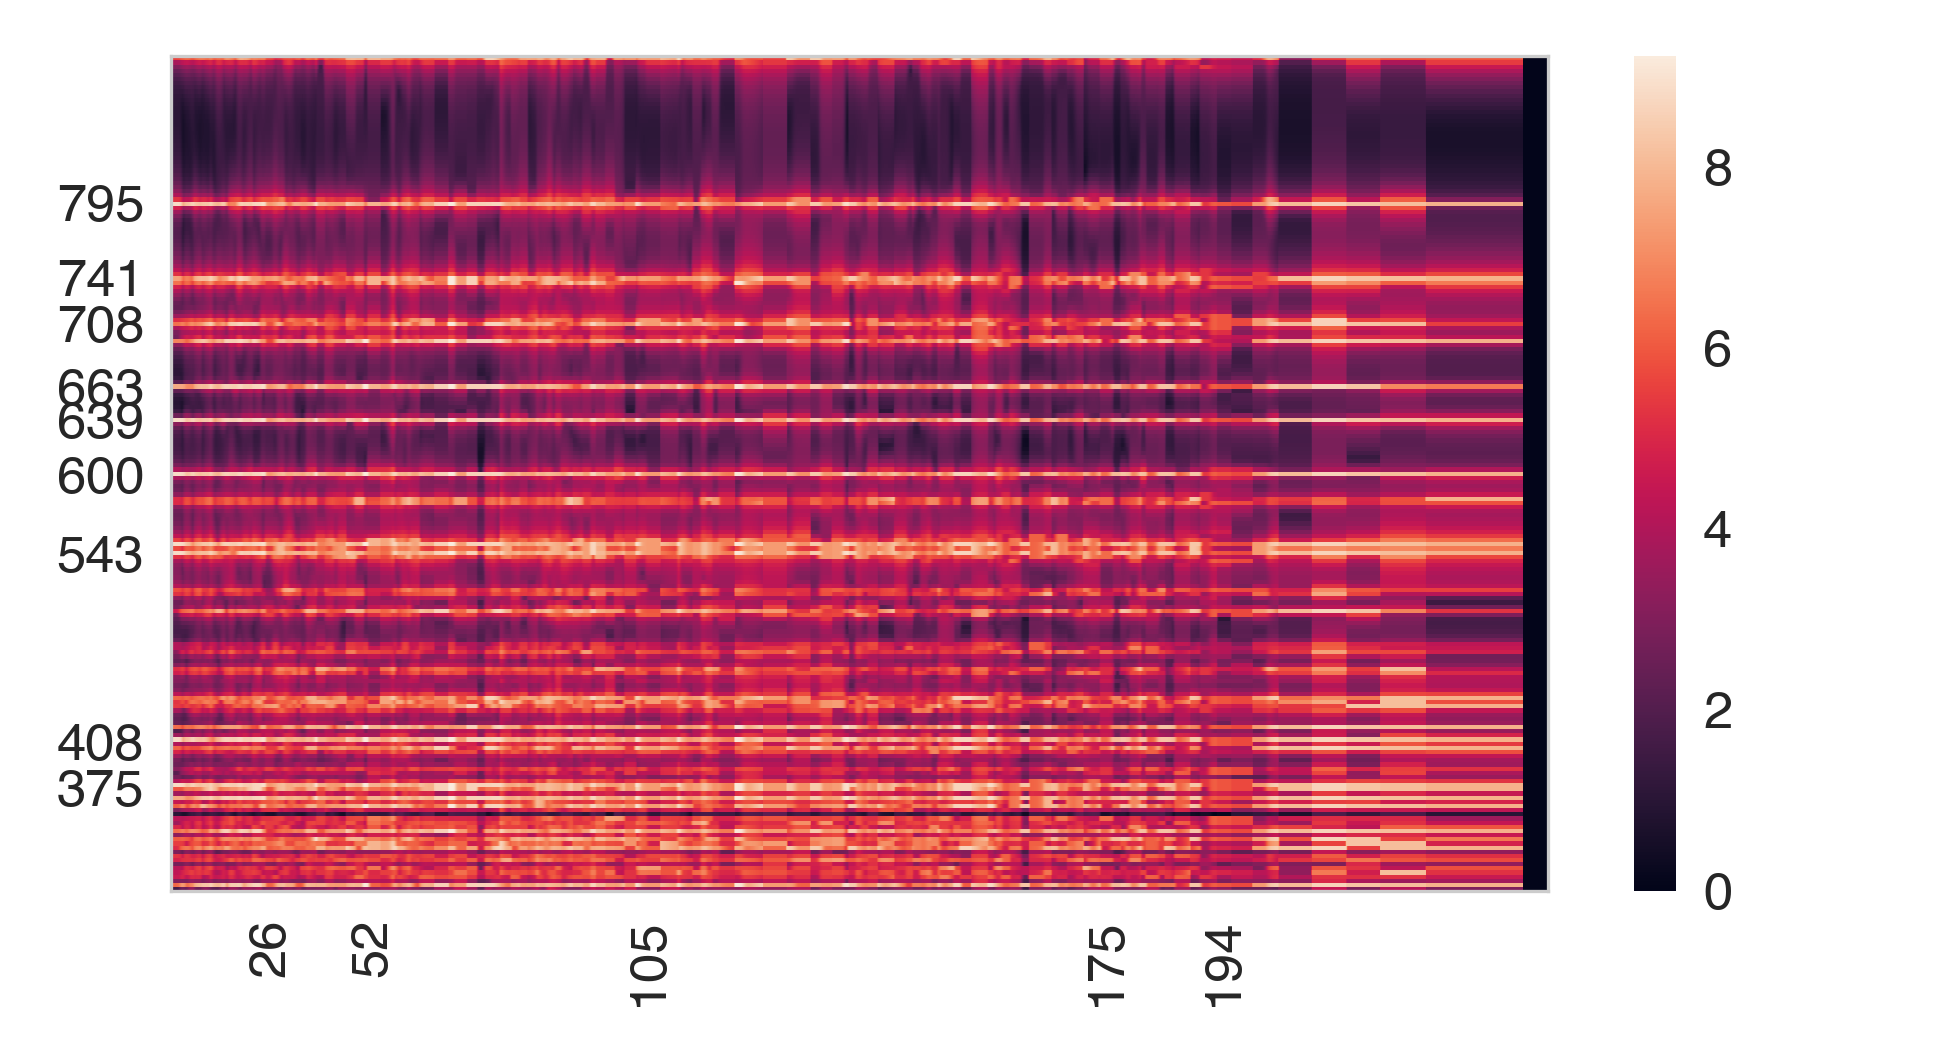
\includegraphics{comb-as12}\caption{Combined graph for As10-STX}\end{subfigure}%
\begin{subfigure}{8.25cm}\centering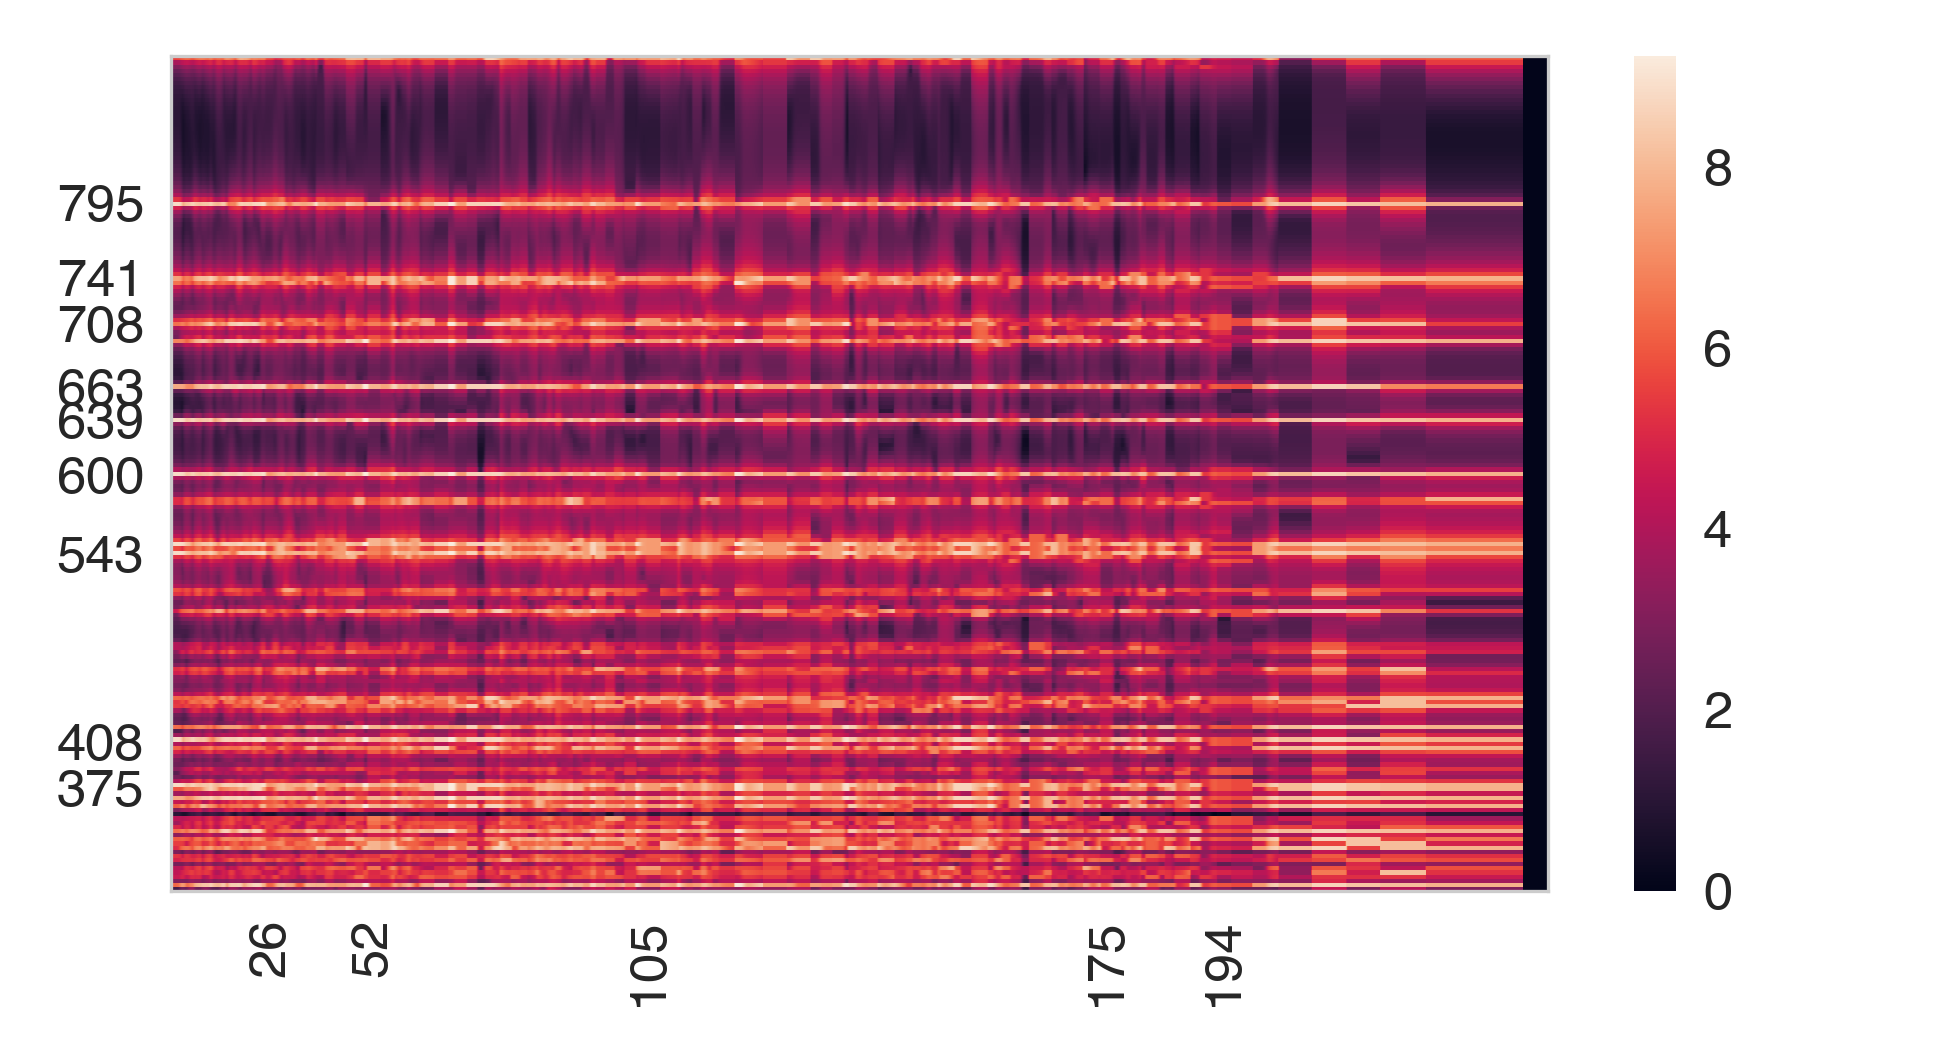
\includegraphics{comb-as12}\caption{Combined graph for As12-STX}\end{subfigure}
\begin{subfigure}{8.25cm}\centering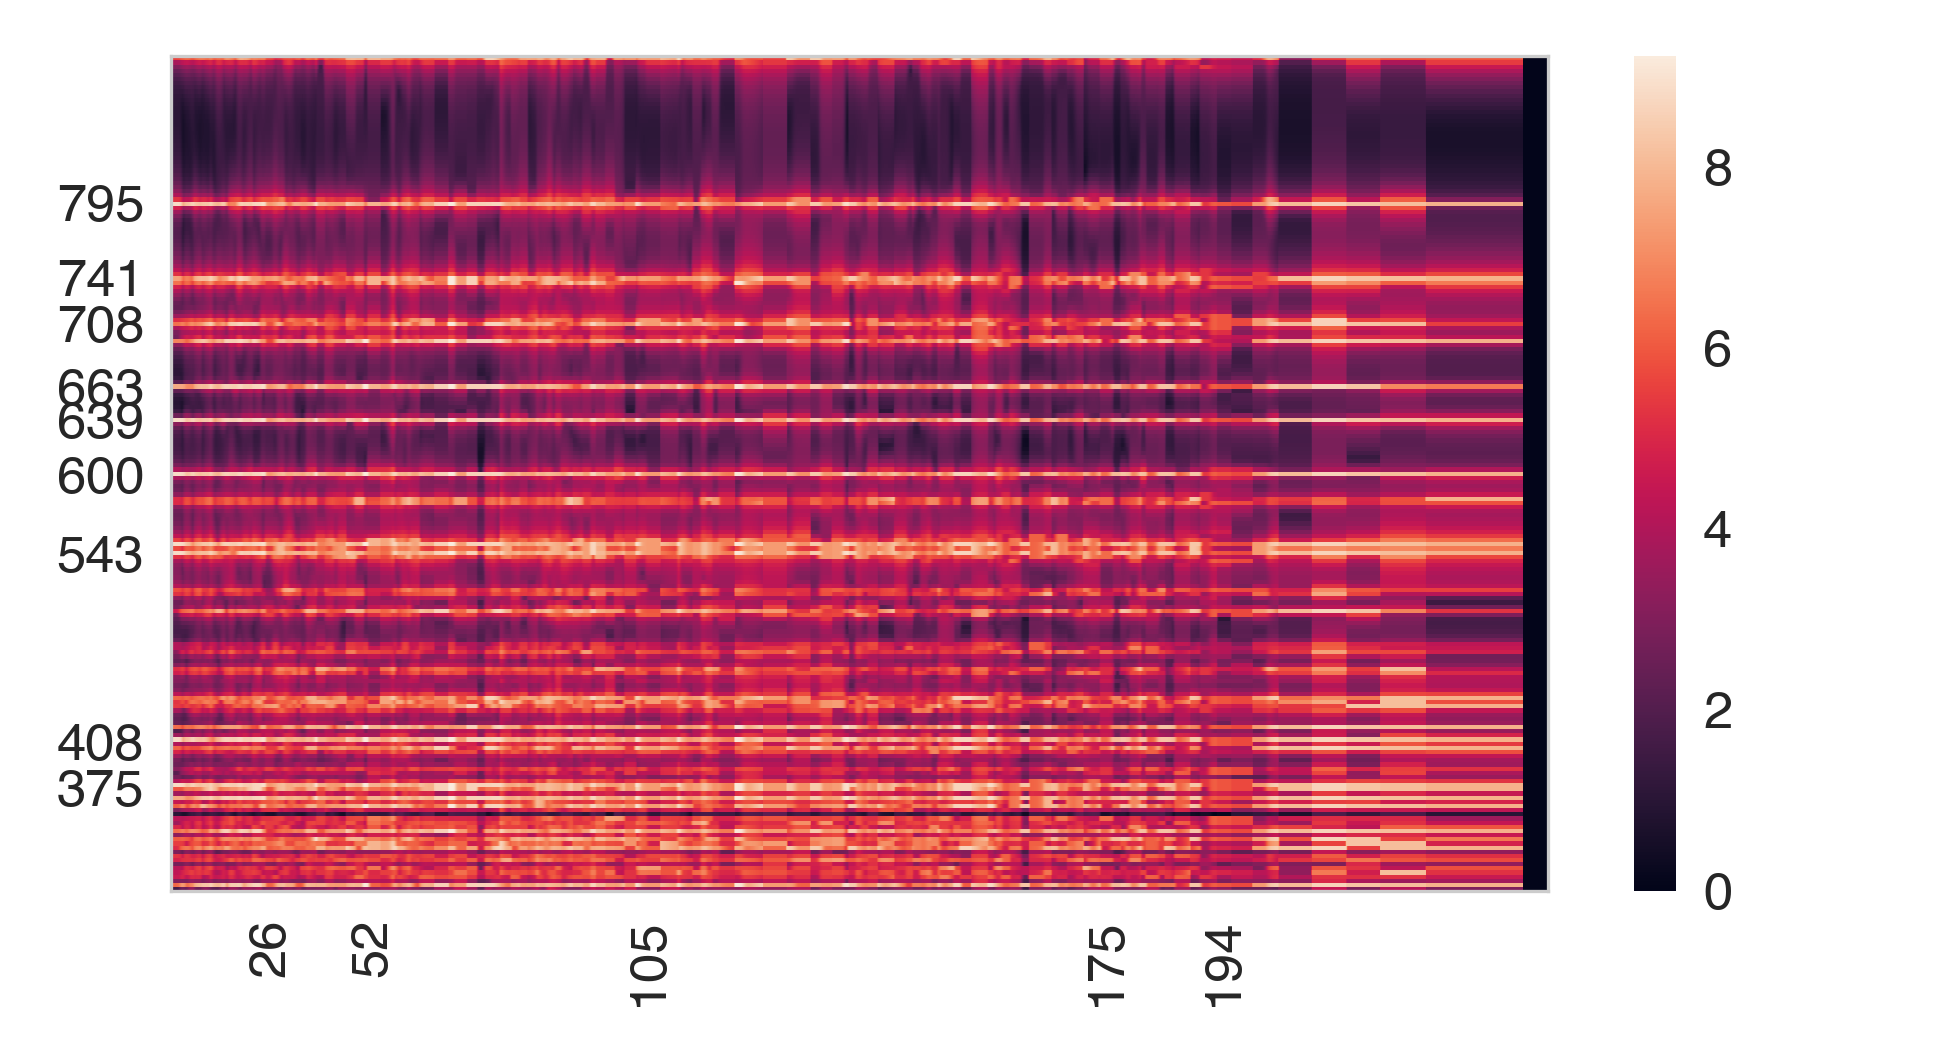
\includegraphics{comb-as12}\caption{Combined graph for AsN08-STX}\end{subfigure}%
\begin{subfigure}{8.25cm}\centering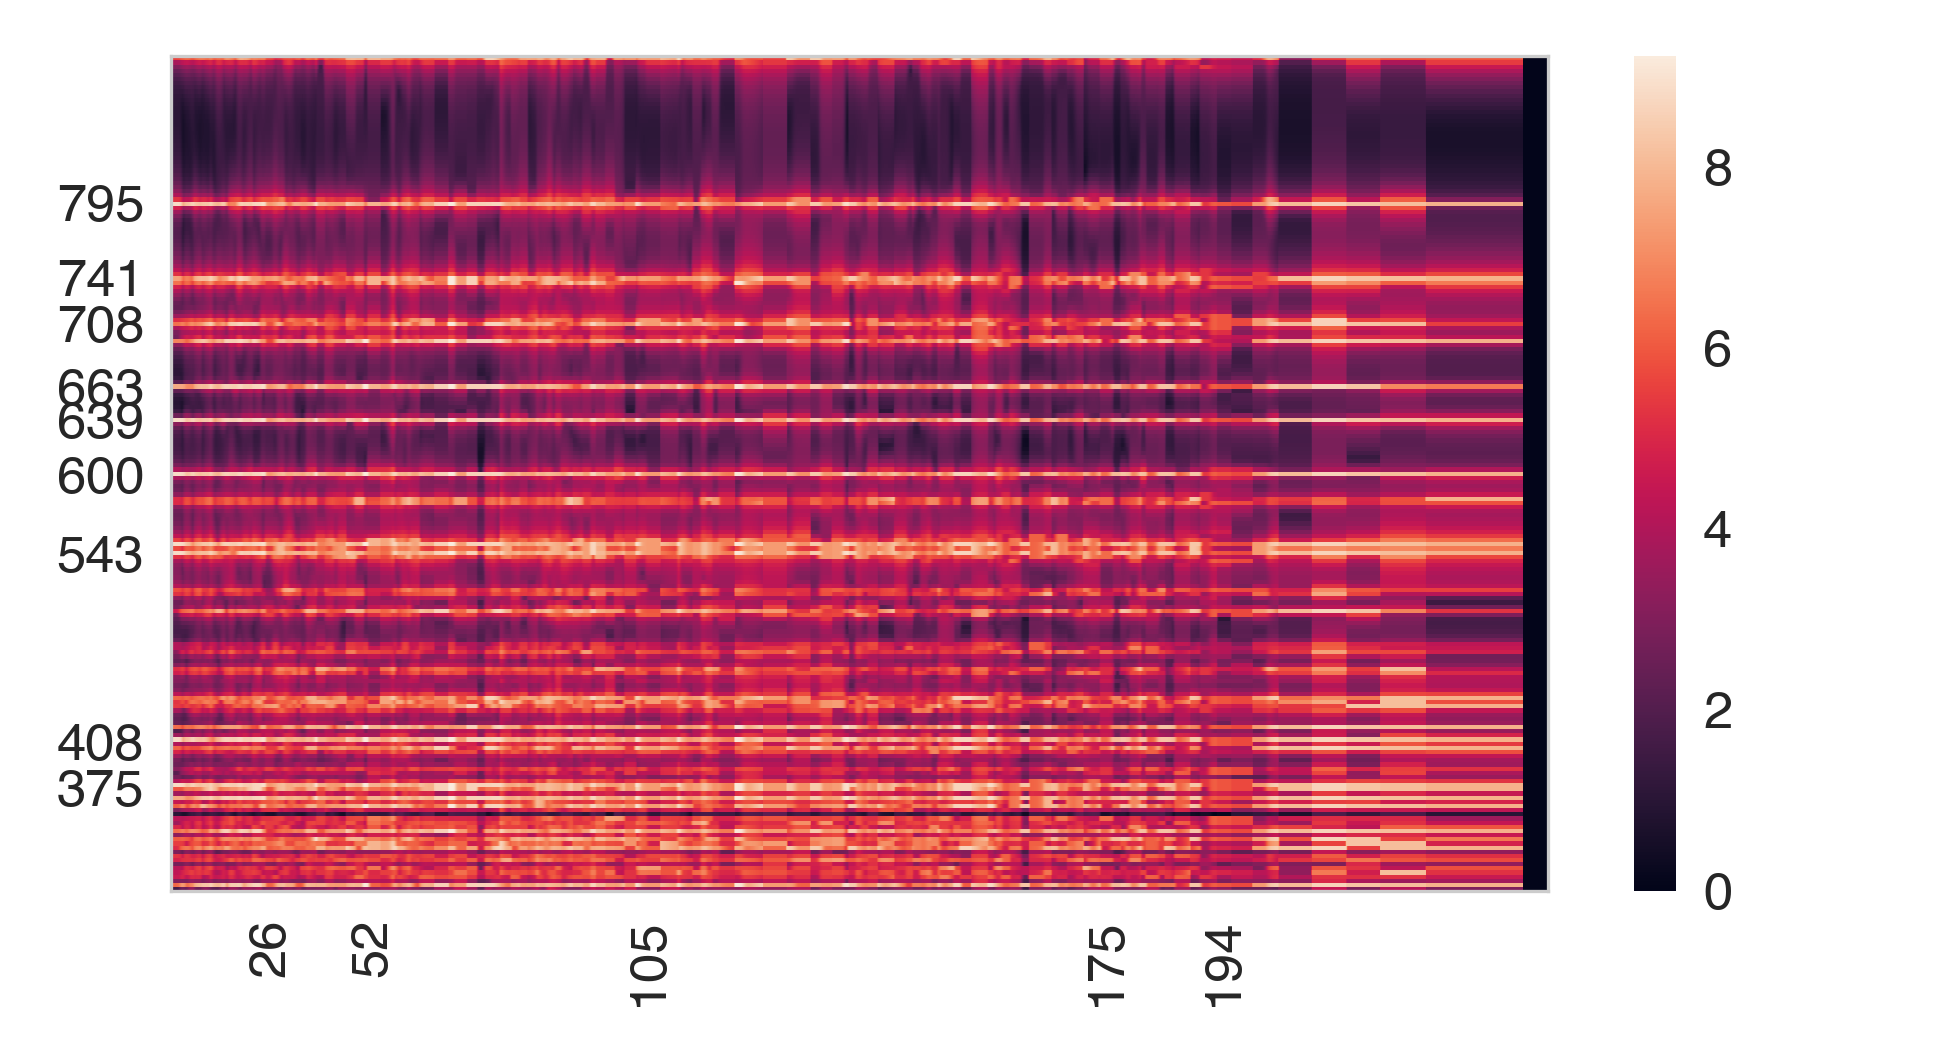
\includegraphics{comb-as12}\caption{Combined graph for AsN10-STX}\end{subfigure}
\caption[Part 1 of combined EF RR graphs]{Part 1 of combined EF RR graphs}
\end{figure*}

\newpage

\begin{figure*}[h]
\centering
\begin{subfigure}{8.25cm}\centering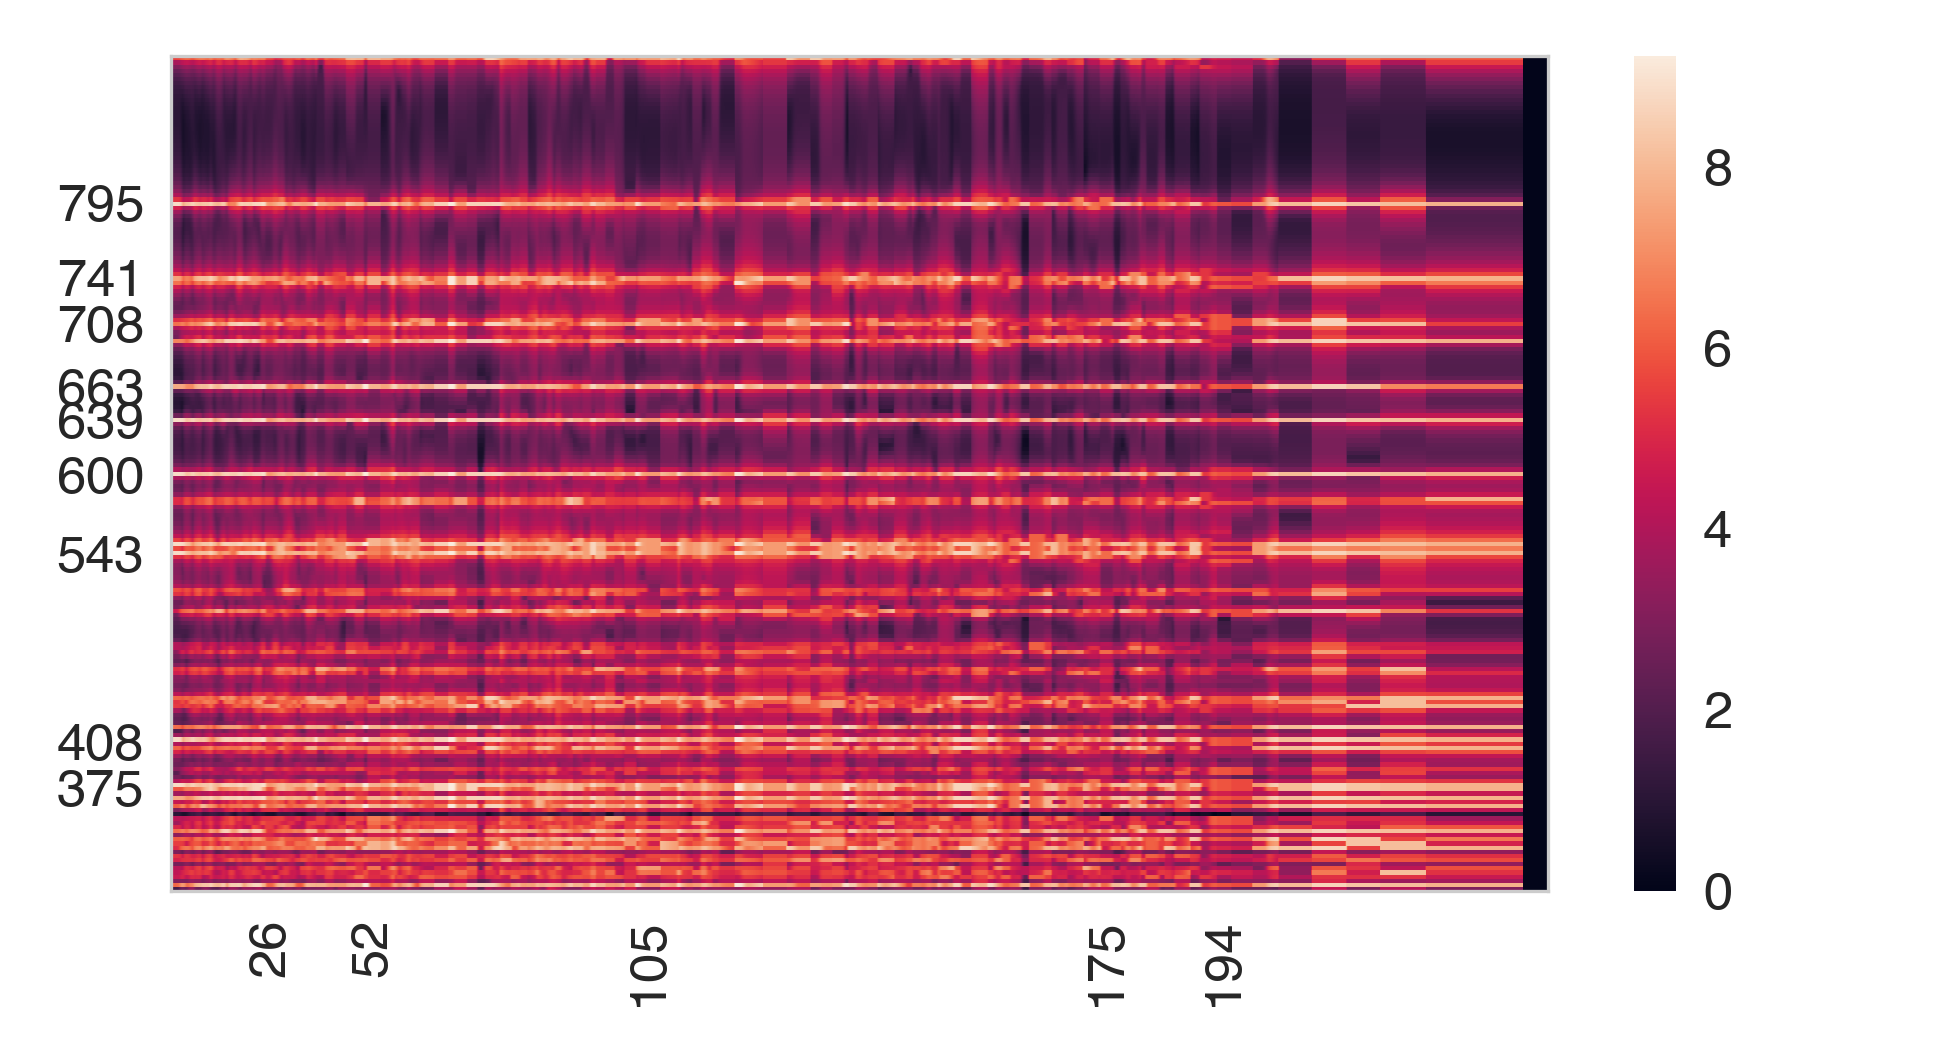
\includegraphics{comb-as12}\caption{Combined graph for AsN12-STX}\end{subfigure}%
\begin{subfigure}{8.25cm}\centering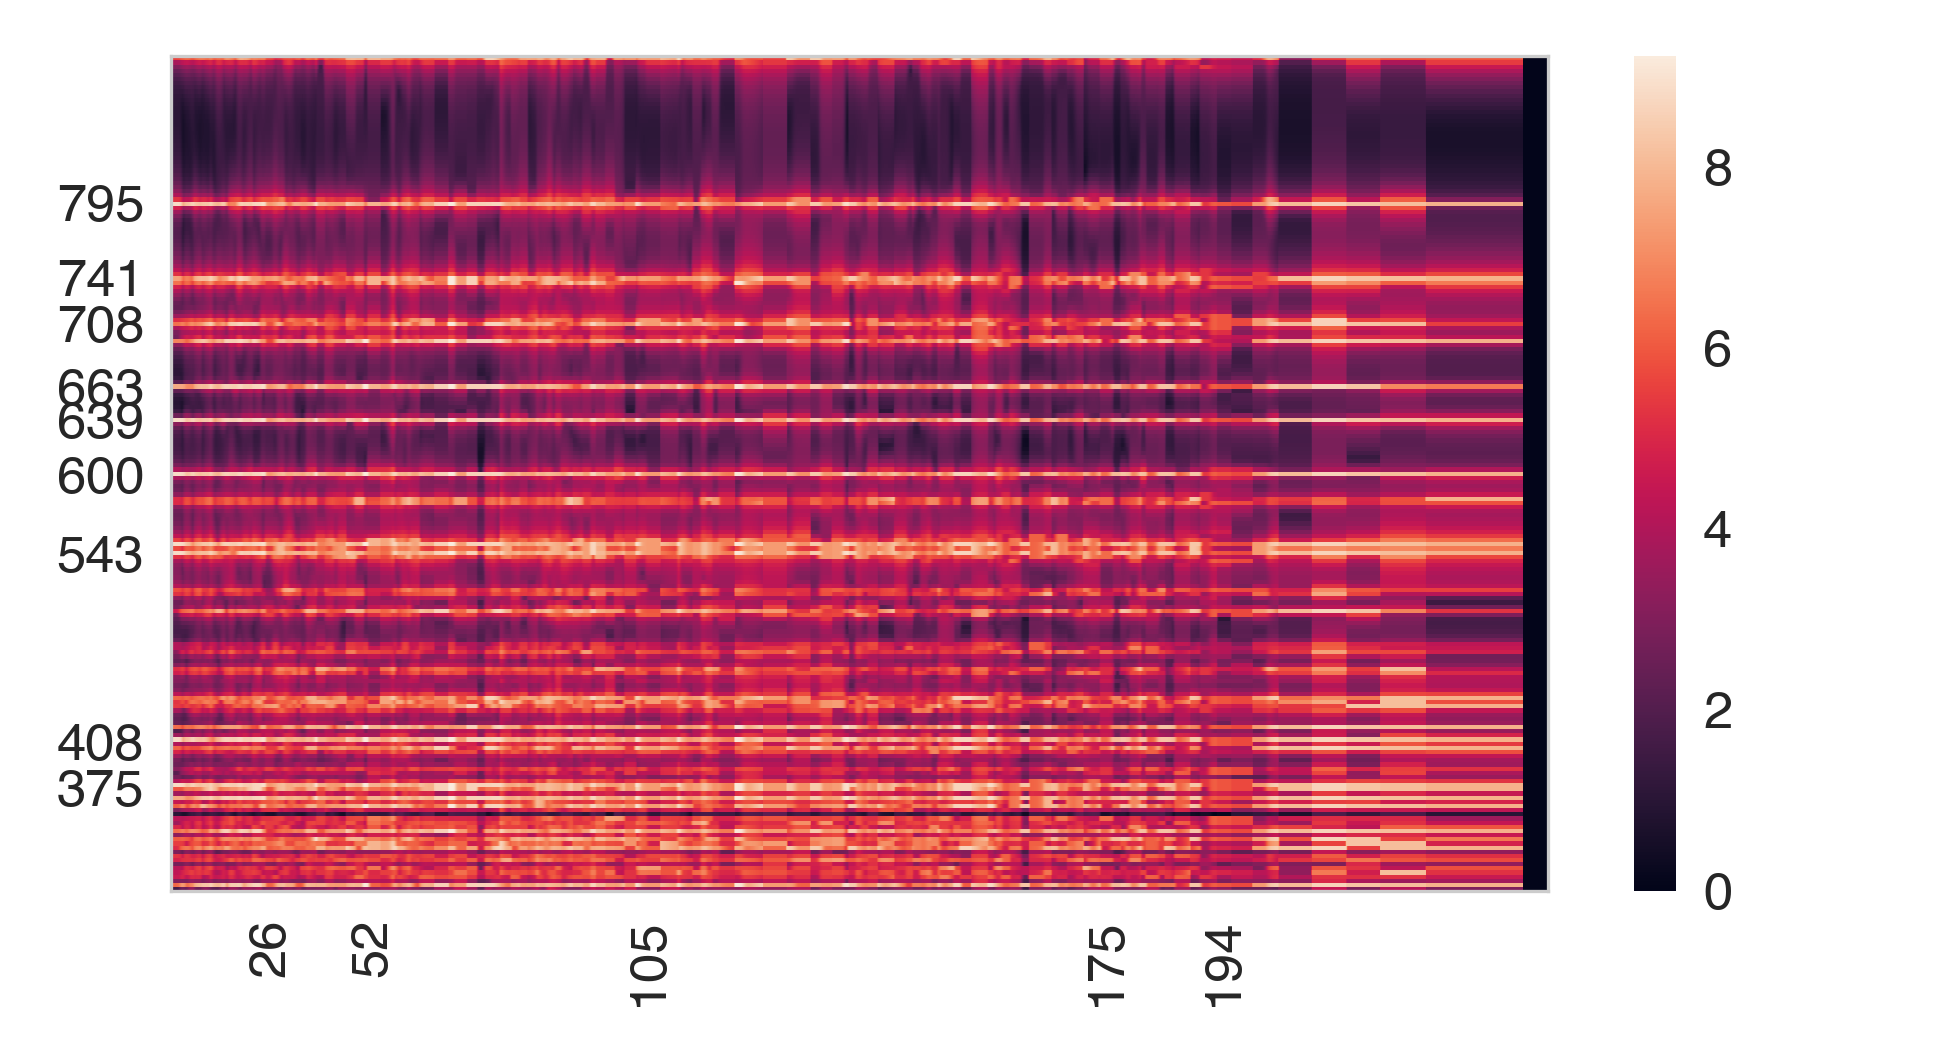
\includegraphics{comb-as12}\caption{Combined graph for P12-STX}\end{subfigure}
\begin{subfigure}{8.25cm}\centering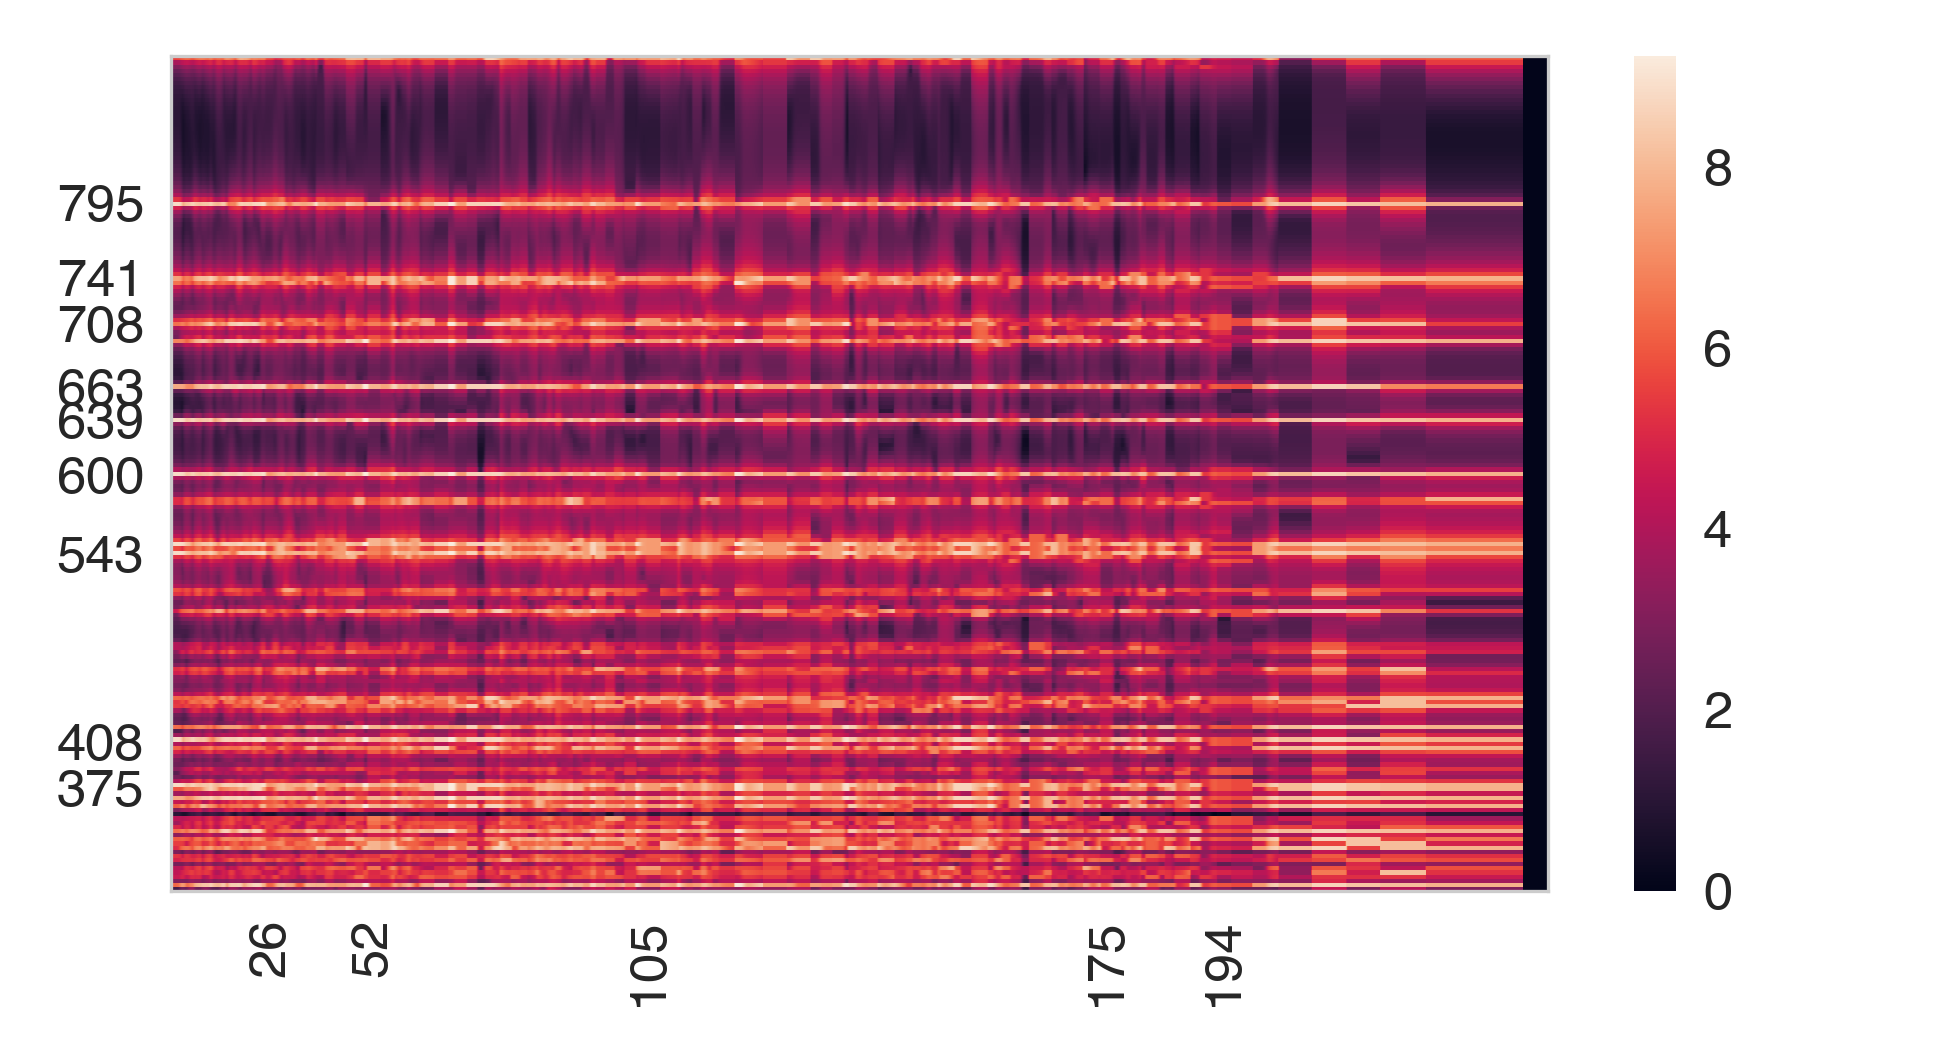
\includegraphics{comb-as12}\caption{Combined graph for PN10-STX}\end{subfigure}%
\begin{subfigure}{8.25cm}\centering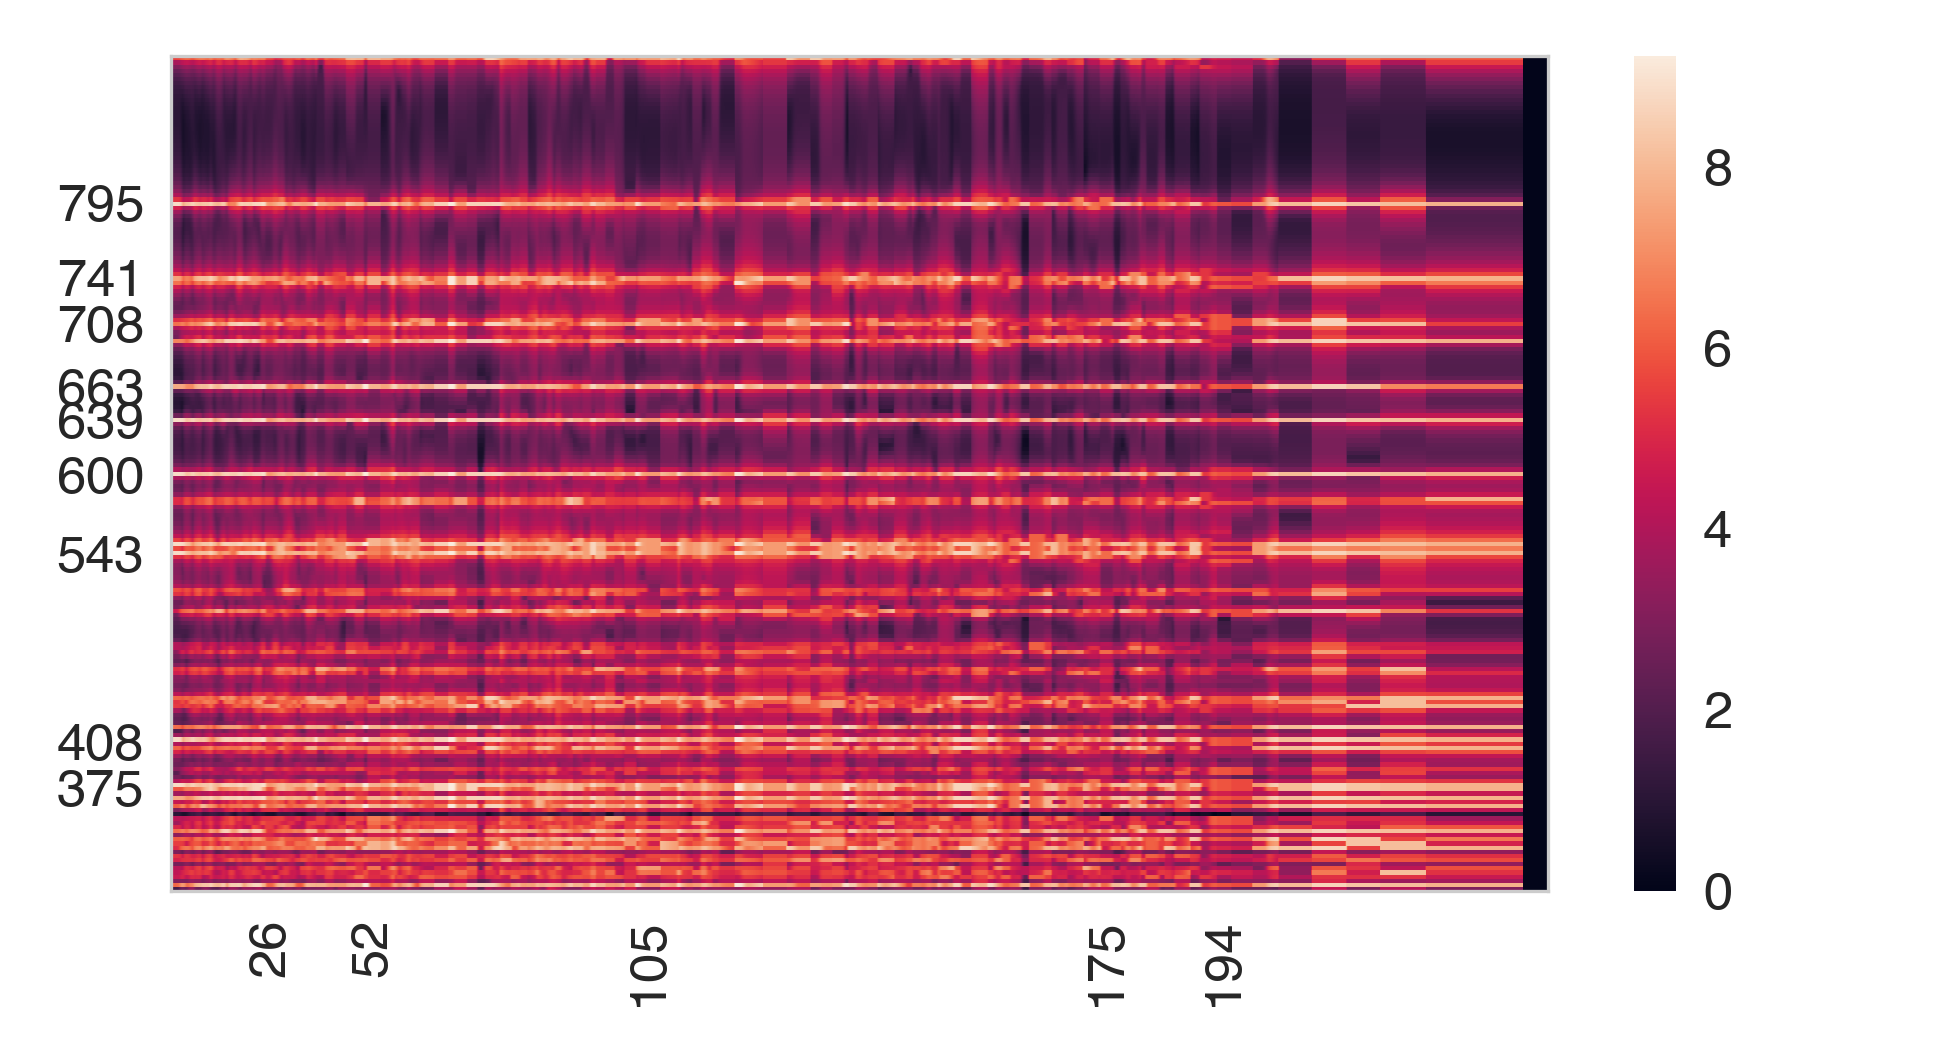
\includegraphics{comb-as12}\caption{Combined graph for PN12-STX}\end{subfigure}
\caption[Part 2 of combined EF RR graphs]{Part 2 of combined EF RR graphs}
\end{figure*}


\newpage
\section{Combined resonance Raman spectra}
